\documentclass[12pt]{article}
\usepackage{amsmath}
\usepackage{amsfonts}
\usepackage{graphicx}
\usepackage{indentfirst}
\usepackage{setspace}
\linespread{1.6}
\usepackage{hyperref}
\hypersetup{
colorlinks=true,
    linkcolor=black,
    filecolor=black,      
    urlcolor=blue,
    citecolor=black,
}
\usepackage[letterpaper, portrait, margin=1in]{geometry}
\usepackage{appendix}
\usepackage{subcaption}

\usepackage{fancyvrb}
\VerbatimFootnotes

\usepackage[para,online,flushleft]{threeparttable}

\usepackage{natbib}
\def\citeapos#1{\citeauthor{#1}'s (\citeyear{#1})}

\title{Habit and skill retention in recycling}
\author{Dylan Brewer and Samantha Cameron\thanks{Brewer (Corresponding author): School of Economics, Georgia Institute of Technology, 221 Bobby Dodd Way, Atlanta, Georgia 30332, \href{mailto:brewer@gatech.edu}{brewer@gatech.edu}.  Cameron: Agricultural and Resource Economics, University of California, Davis, 2116 Social Sciences and Humanities, University of California, Davis, One Shields Avenue, Davis, CA 95616, \href{mailto:sjcameron@ucdavis.edu}{sjcameron@ucdavis.edu}.  We thank Stefano Carattini, Matt Oliver, Jonathan Scott, Keith Teltser, Casey Wichman, Daniel Dench, Cody Orr, and seminar participants at the Southern Economics Association and Midwestern Economics Association conferences for useful discussion and feedback. Replication package available at \href{https://github.com/dylanbrewer/RecyclingHabits}{https://github.com/dylanbrewer/RecyclingHabits} or \href{https://doi.org/10.5281/zenodo.8292759}{https://doi.org/10.5281/zenodo.8292758}. The authors declare no known conflicts of interest.}}
\date{\today}

\begin{document}

\maketitle

\begin{abstract}
\begin{singlespace}
\noindent
From 2002-2004, New York City ceased collecting residential glass and plastic recycling due to city budgetary pressure.  We use data on recycling rates in New York City, New Jersey, and Massachusetts in a difference-in-differences (DID) research design to determine whether this exogenous pause weakened previously formed recycling habits.  Despite a 50\% decline in the overall recycling rate in 2003, by 2005 the overall recycling rate had fully recovered.  Our results suggest that recycling habits are persistent in the short term and that the loss of previously established recycling habits and skills are not an unintended harm of pausing a recycling program.  We show that these results hold in the standard DID approach, as well as a synthetic DID approach modified to estimate time-disaggregated treatment effects separately, which eliminates pre-trends and improves the precision of our estimates.
\end{singlespace}
\end{abstract}
\noindent \textit{Keywords}: Recycling, waste, learning by doing, habit formation, synthetic difference in differences

\noindent \textit{JEL codes}: D83, H40, Q53, Q58

\clearpage

\section{Introduction}

Learning from experience and habit formation are often key inputs in the design of public policies.  For example, the successful adoption of new technologies, practices, and policies may require experience which accumulates through persistent use in a learning-by-doing process \citep{fosterrosenzweig1995}.  Policy interventions can also create persistent effects or habits that, when unaccounted for, can lead to underestimation of the intervention's impact \citep{allcottrogers2014}.  Repeated interventions can potentially enforce habits or can cause the targets to become habituated (desensitized) to the policy intervention \citep{itoidatanaka2018}.  Furthermore, it may be cost-effective to pursue a policy at a loss in the short run if it creates skills or habitual capital with value in the future.

Municipal recycling is one widely adopted policy that many argue creates valuable skills and habitual capital for future use.  Residential recycling provides environmental benefits and makes people feel good, but it is also costly and has a low success rate due to residual food waste.  To illustrate, municipal programs recycled 40 million tons of residential waste in 2019 in the United States at a cost of around \$80 per ton for collection and processing. In 2017, the value of an average ton of recyclable materials was \$90 per ton, but by 2019 the value had fallen to \$40 per ton, leaving a \$40 net accounting cost per ton \citep{mouwetal2020}, which can be more costly than landfill disposal in some states \citep{kantnerstaley2019}.  After considering external benefits and citizen willingness to pay, the net benefit of most municipal recycling programs are close to zero, although this varies by municipality and depends substantially on the value of raw materials \citep{aadlandcaplan2006}. Despite these challenges, recycling is very popular in the United States, with municipal recycling programs operating at a \$2 billion accounting loss in 2019 \citep{mouwetal2020}.  

One popular argument leveraged in favor of continuing to recycle despite high costs posits that recycling programs should be maintained so that when the value of materials increase or new technology makes recycling profitable, households are well-practiced at separating recyclable from non-recyclable waste.  For example, in response to the rising costs of recycling in 2019 and the practice of collecting recycling separately to send to a landfill, one municipal recycling manager stated in a \textit{Los Angeles Times} interview that ``A lot of people have built up good recycling habits in recent years, and we want them to keep up those habits'' \citep{latimes2019}.  When faced with the prospect of pausing recycling collection, another recycling manager expressed the fear that it would be difficult to ``retrain'' people to recycle in the 2019 NPR \textit{Planet Money} episode ``So, Should We Recycle?" \citep{planetmoney2019}.  These arguments posit that an increase in recycling today will create value through increased recycling tomorrow in a persistent dynamic process.

A habit is a default or automatic behavior that develops through repetition and is closely related to learning and skill formation \citep{woodrunger2016}.\footnote{\cite{alpizaretal2022} point out that habit formation and learning-by-doing occur via similar theoretical assumptions of exposure-enhanced consumption or behavior.} Both households and waste management entities may develop skills and habits that may cause dynamic persistence of recycling.  First, recycling is a behavior that becomes easier over time as individuals develop habitual capital that lowers the costs of complying---people learn which items may be recycled and default to recycle certain types of goods habitually.  Second, the waste management entity develops its own institutional capital by repetition---reducing its cost of recycling in subsequent periods.  This may involve purchasing physical capital such as recycling trucks, hiring necessary labor to accommodate the additional pickup, or developing operational and managerial expertise.  Thus, for individuals and recycling management entities, past recycling reinforces future recycling and forms habitual capital stock, consistent with the theoretical mechanisms driving learning-by-doing and habit formation.

The cessation of a recycling program may cause habits and skills for households and recycling management entities to degrade.  Households may need to relearn which materials are recyclable or redevelop waste-sorting practices.  Depending on the length and scope of the pause, the recycling management entity may divest physical recycling capital, such as recycling trucks, and cut employment.  Similarly, managerial and operational expertise degrades over time.

In this paper, we study a natural experiment that allows us to evaluate the degree to which recycling habits and skills form and are lost or retained in response to a temporary pause in municipal recycling.  Residential recycling has been mandatory in New York City since 1989 \citep{lubasch1989,macbride2004}.  However, in 2002 budgetary pressure spurred the Mayor and City Council of New York City to order an indefinite cessation of the collection of residential glass and plastic recycling.  From July, 2002 through April, 2004, the Department of Sanitation of New York City (DSNY) did not collect residential glass and plastic recycling \citep{macbride2004}.  DSNY continued to collect paper and metal recycling.  Commercial entities continued to contract with private waste removal services with no changes during this period.  We take advantage of this pause to measure whether, and to what extent, recycling skills and habits degraded.

To evaluate the effect of the pause in recycling, we compare data on recycling rates in New York City boroughs with control regions in Massachusetts and New Jersey in a difference-in-differences (DID) research design.  The outcome variable, recycling rate, is the fraction of waste diverted for recycling, including metal, glass, plastic, paper, and organic recycling.  Our preferred approach uses a modified synthetic DID procedure to estimate time-disaggregated treatment effects of the pause on recycling rates over time \citep{arkhangelsky2021}.  Our synthetic DID procedure estimates different time and unit weights to calculate each post-treatment period estimate in a stacked approach.\footnote{The ``stacked'' terminology is imported from the staggered event-study approach taken by \cite{cengizetal2019} which separately estimates effects for treatment cohorts.  In this paper, all units are treated at the same time, but we estimate treatment effects for each post-treatment time period separately.}  The stacked synthetic DID weights differ relative to using the entire post-treatment period to calculate weights, although in our context the point estimates from either approach are roughly the same.  We show that the traditional synthetic DID time weights with multiple post-treatment periods are the average of the stacked weights estimated separately for each post-treatment period.  The main advantage is that the stacked approach substantially increases the precision of the estimates due to re-estimation of the time weights for each treatment effect estimate.  

In our empirical context, synthetic DID has distinct advantages relative to a DID event-study (e.g., \cite{borusyakjaravel2018}) or synthetic control estimation (e.g., \cite{abadie2021}).  The standard identifying assumption of parallel trends in the evolution of the recycling rate between control and treatment appears unlikely to hold, thus casting doubt on a standard event-study.  Further, it is difficult to construct a convincing synthetic control because only five years of pre-treatment data exist and the recycling rate in New York City is low relative to most of the control units, which can make it difficult for the synthetic control approximate \citep{abadie2021}.  In contrast, synthetic DID produces a weighted control group with parallel trends in the recycling rate between treatment and control groups during the pre-period.  In our empirical context, synthetic DID produces more precise but similar estimates to the event study, while the synthetic control suffers from general lack of precision.

The 2002-2004 pause in glass and plastic recycling reduced recycling rates in those years substantially, but by 2005 New York City's recycling rate had fully recovered.  We estimate that the pause reduced yearly recycling rates by 6.5, 9.7, and 3.1 percentage points in 2002, 2003, and 2004 compared to the control regions.  Relative to an average pre-pause New York City recycling rate of 18.3\%, this was a reduction of more than 50\% in 2003.  Our synthetic DID estimates indicate a full recovery in recycling rates after the pause was lifted. In 2005, the first full year that recycling resumed, we find that New York City's recycling rate was 0.06 percentage points \textit{higher} than the synthetic DID counterfactual prediction. From 2006 to 2008, recycling rates were unaffected by the pause.  The finding of a quick rebound in recycling is consistent with persistent skills and habits in recycling.

Our results are relevant to policymakers considering whether to discontinue an unprofitable arm of a municipal recycling program.  This natural experiment suggests that recycling rates can recover quickly, at least when the pause is short and other municipal waste services continue.  The quick recovery implies that policymakers need not be concerned that recycling rates will take a long time to rebuild. We further discuss the generalization of our results to other municipal contexts and argue that the details of the pause in New York City are important to consider.

The next section reviews related literature on habit formation and recycling. Next, we introduce an informal theoretical framework, data, and suggestive evidence on habit and skill formation and decay.  We then introduce our stacked synthetic DID research design and present our empirical results.  Finally, we conclude and discuss the generality of the results to other policy contexts.

\section{Previous research}

Most empirical work in the habit-formation and learning-by-doing literature only observes the end of an intervention---ours is a unique contribution in that we observe behavior both during an indefinite pause in the intervention and after it resumes again.  For example, \cite{bechteletal2018} study the repeal of a mandatory voting in a Swiss Canton, finding little evidence for habit formation as voting rates quickly dropped.  Diet and exercise habits are a common subject of study in this literature, with research showing that long-lasting behavioral changes can result from short-term food price changes and costs of exercising.  \cite{atkin2013} derives a model showing that low-priced foods during childhood may remain persistent food choices due to habit formation, finding evidence to support his hypotheses in Indian regional food price and consumption data.  \cite{HARRIS2019} find that when exercise sessions are missed due to an exogenous event like rainfall, individuals are less likely to exercise in the future, suggesting that frequent reinforcement is important in habit formation. In some contexts, emphasizing healthy food menu highlights lead to continued healthy food choices after the intervention, while in other contexts behavior quickly reverts to the norm.  A menu intervention highlighting vegetarian food options at a restaurant resulted in increased consumption of vegetarian food after the menu reverted back to normal \citep{KURZ2018}. However, a similar intervention highlighting healthy food in a school cafeteria did not have persistent effects on children's food choices after the intervention ended \citep{OZTURK2020}, suggesting the institutional context is an important factor in whether such effects are observed.  

Several household energy consumption studies show that nudges to conserve energy reduce consumption beyond the nudge period due to changed behaviors, adoption of energy efficient appliances, and inertia due to the cost of altering thermostat settings.  \cite{allcottrogers2014} observe that households who receive home energy reports reduce energy consumption and appear to develop habits that last beyond the intervention period due to adoption of new behaviors and energy-efficient appliances.  Similarly, \cite{brewercrozier2022} show that the effects of emergency requests to reduce thermostat settings persist beyond the emergency period, creating a short-lived persistent effect due to inertia. \cite{itoidatanaka2018} find that households become habituated to repeated nudges for energy conservation but that price incentives appear to result in more persistent conservation behavior.

In the environmental psychology and psychology of habit formation literature, there has been limited work regarding the psychology of starting and retaining recycling behaviors \citep{nordlund2011}. Existing work on recycling psychology focuses mainly on the correlation between pro-environment attitudes and resulting pro-environment behavior.  In the context of paper recycling, \cite{mcguinness1977attitudinal} find that attitudes (including beliefs, intended action, and knowledge) toward ecology and paper recycling has a significant relation to paper recycling participation.  In a survey, \cite{knussenyule2008} find that respondents with either a history of past recycling or a self-assessed habit of recycling were more likely to recycle. Moreover, evidence of others’ recycling behaviors will have a positive impact on an individual’s recycling habits \citep{topf2023follow}. \cite{ouellette1998habit} find that the most important determinants of the strength of habits are frequency of past behaviors, the degree to which the individual initially learned the behavior, and the environment in which the behavior occurs. Attitudes toward the desired behavior are also very important in determining the existence and persistence of actions \citep{ouellette1998habit}. Generally, as awareness of environmental consequences of a behavior increases, so does the formation of pro-conservation habits \citep{gregory2003repeated}. When coupled with regular reinforcement (e.g. daily practice of habit rather than monthly), awareness and attitudes can help to form strong and lasting habits \citep{gregory2003repeated}.  Our paper provides novel natural field experimental evidence to this literature, and we believe is one of the few examples of causal inference methods to study a natural experiment related to recycling habits.

Finally, this paper contributes the first study on recycling habits and skills to the economics literature on waste and recycling.  The economics literature on waste and recycling focuses substantially on per-unit waste pricing, typically finding that per-unit pricing of waste incentivizes reductions in waste generation and substitution toward recycling \citep{fullertonkinnaman1996,fullertonkinnaman2000,usuitakeuchi2014,carattini2018,wright_halstead_huang_2019,buenovalente2020}.  Another strand of the literature studies the determinants of pro-environmental behavior such as recycling using surveys and stated-choice methods.  \cite{viscusihuberbell2011} find that state recycling laws, personal beliefs, and income increase respondents' survey-reported likelihood of recycling. \cite{czajkowskietal2017} provide evidence that characteristics of the recycling program (such as where recycling is sorted) matter for participation.  \cite{kipperberglarson2012} find, using a stated-choice experiment, that households in Seattle had a positive willingness to pay for increases in the community recycling rate.  Our paper is unique in this literature for its focus on habits and skills while leveraging a natural experiment for identification.

\section{Theoretical framework, data, and suggestive evidence}

Both household recycling behavior and institutional collection of recycling exhibit characteristics of path dependence that are consistent with habitual capital formation or learning-by-doing.  \cite{beckermurphy1988} show that when an action is less costly than when that same action was performed in a previous period, rational agents can develop self-enforcing habits (or addictions).  \cite{fosterrosenzweig1995} document how individuals develop human capital skills from repeated actions or practice.  When an individual recycles for the first time, there may be costs to learning.  Simply remembering that recycling is an option becomes easier over time.  Beyond simple memory, which types of plastic are recyclable?  Should glass and metal be separate?  Does recycling pickup happen on trash pickup day or the day after?  Each subsequent week, these costs are lower and a habit begins to form.  Similar mechanisms occur for the recycling entity.  Managerial and operational expertise grows over time, creating an institutional capital stock that may result in increased recycling rates.  A pause in the recycling program may cause habitual and institutional capital to degrade as acquired habits and skills fall out of practice.

On the extensive margin, information about a new recycling program takes time to diffuse, and take-up rates may be low at first.  In a diverse city like New York, language barriers may exacerbate this problem.  For the recycling entity, it may take time to assemble the physical recycling capital and employment necessary to collect all recycling.  During an extended pause, the city may divest physical recycling capital and cut recycling employment.  Purchasing and hiring may take additional time to complete upon restarting.

We hypothesize that the opportunity cost of a pause in recycling includes the foregone recycling during the pause, the foregone habits, skills, and institutional capital that will lead to reduced recycling in the future, and the expected start-up costs of resuming service.  If this hypothesis is correct, an interruption in recycling activity would cause reductions in recycling during the pause and persistent reductions in recycling after the pause because of lost habits and skills.  We evaluate our hypothesis by examining a pause in recycling collection in New York City between 2002 and 2004.

The Department of Sanitation of New York City (DSNY) is responsible for residential waste management, recycling, and snow removal in the city.\footnote{Commercial entities contract with private contractors to remove commercial waste \citep{dsnycommercial}.}  Recycling has been mandatory in New York City since 1989.  We obtain administrative data on monthly waste removed by DSNY at the community district level from 1997 to 2008 from New York City's open data portal \citep{dsnydata}. We aggregate our data to the borough level and restrict our analysis to the Bronx, Brooklyn, and Queens boroughs because DSNY stopped recording tons of paper recycling from Manhattan and Staten Island from 1998-2004.\footnote{According to DSNY's 2002 annual report, paper collected in Manhattan and Staten Island were directly taken to Visy Paper, a recycling company, which may explain why paper recycling was not recorded.  Including Manhattan and Staten Island in the sample would cause the recycling rate in those boroughs to increase artificially in 2004, so we take the conservative approach of dropping them from the sample.}  To match the control data, we construct the recycling rate as the fraction of tons diverted for recycling and composting divided by total tons of residential waste.

For control units, we obtain data on yearly residential recycling rates in Massachusetts municipalities and New Jersey counties from 1997 through 2008.  Our choice of controls is limited by the lack of widely available recycling data from the 1990s, but Massachusetts and New Jersey contain large urban centers that are similar to New York City in culture, political affiliation, and income, making these states viable control groups.\footnote{A natural control group would be other large US cities, but we were unable to find data in other large cities with information on recycling with a sufficient pre-period before the pause in 2002.} Massachusetts data come from the Massachusetts Department of Environmental Protection's Municipal Residential Recycling Rate survey \citep{massdata}.  In Massachusetts, each recycling program is managed at the municipality level, may either be mandatory or voluntary for residents \citep{massmandatory2021}, and often requires sorting similar to New York City's program.\footnote{In Massachusetts, hazardous products diverted from the waste stream are also counted in the recycling tonnage (e.g., car batteries). In 2003, the first year where recycling type is delineated by category, hazardous products is just 1.4\% of total recycling tonnage.}  New Jersey data come from the New Jersey Department of Environmental Protection \citep{njdata}, where recycling has been mandatory at the state level since 1987 \citep{njlaw}. Each New Jersey municipality separately manages recycling and has different requirements and processes.  For each state, we include only regions that reported continually operating a recycling program during this period.  The final control group includes 186 Massachusetts municipalities and 21 New Jersey counties observed from 1997-2008.

\begin{figure}
\centering
\begin{subfigure}[c]{.49\textwidth}
    \centering 
    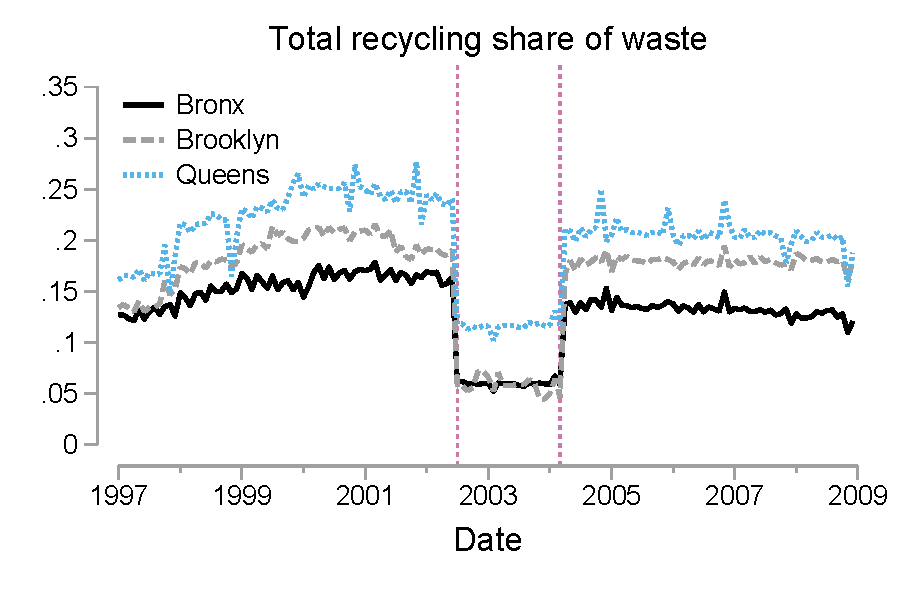
\includegraphics[width=\linewidth]{rrtrends.pdf}
            \caption{}\label{fig:rrtrends}
    \end{subfigure}
\begin{subfigure}[c]{.49\textwidth}
    \centering
    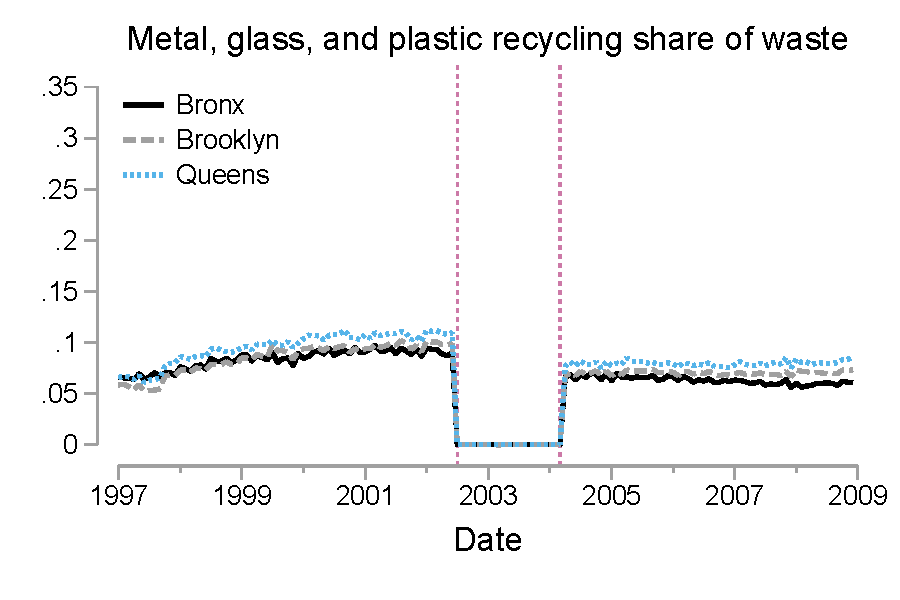
\includegraphics[width=\linewidth]{mgptrends.pdf}
        \caption{}\label{fig:mgptrends}
\end{subfigure}

\medskip

\begin{subfigure}[c]{.49\textwidth}
    \centering
    \vspace{0pt}
    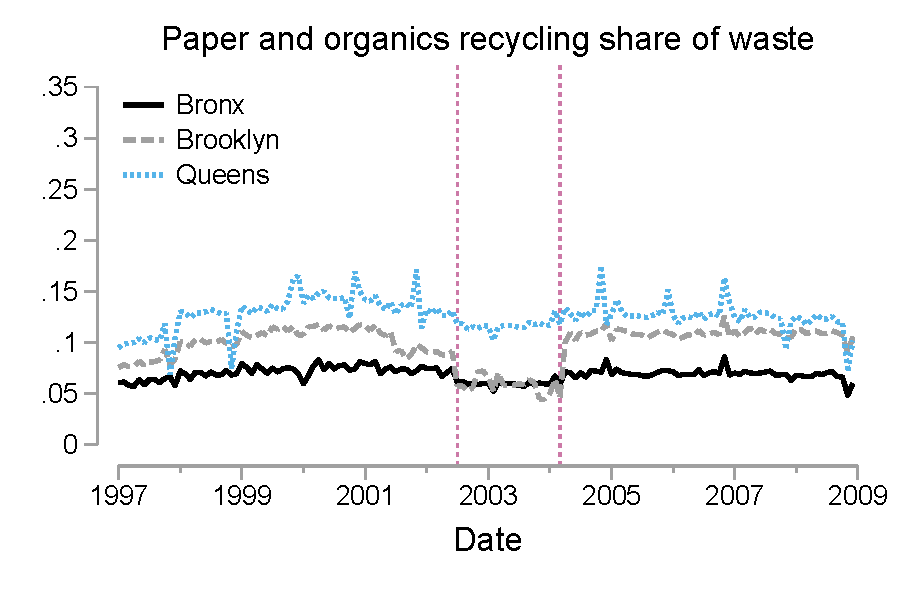
\includegraphics[width=\linewidth]{othertrends.pdf}
        \caption{}\label{fig:othertrends}
\end{subfigure}
\begin{subfigure}[c]{.49\textwidth}
    \centering
    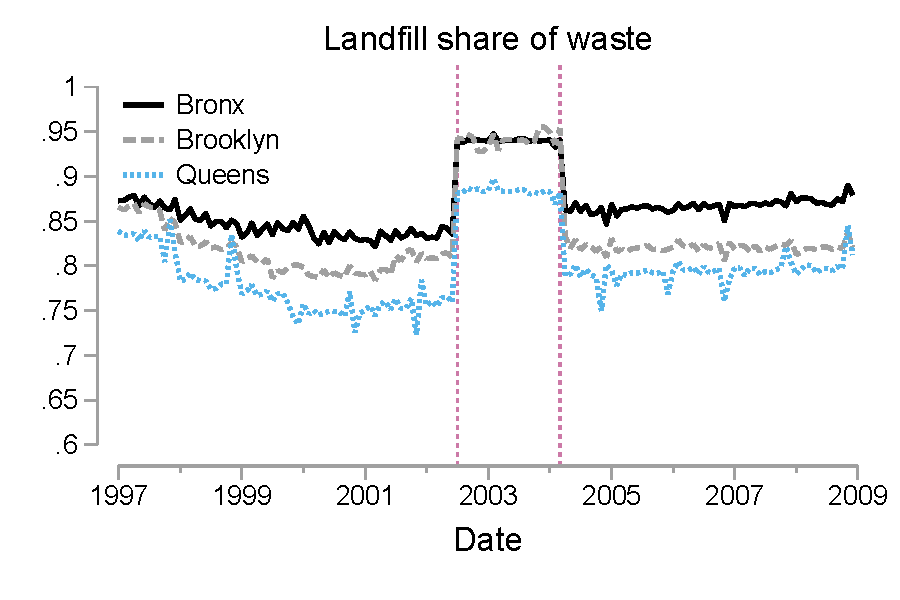
\includegraphics[width=\linewidth]{refusetrends.pdf}
        \caption{}\label{fig:refusetrends}
\end{subfigure}
    \caption{Deseasonalized fraction of all waste recycled monthly by type in New York City.  Red vertical lines delineate the pause in glass and plastic recycling collection.  Panel (\subref{fig:rrtrends}) plots the share of all recycling, panel (\subref{fig:mgptrends}) plots the share of all metal, glass, and plastic recycling, panel (\subref{fig:othertrends}) plots the share of paper and organics recycling, and panel (\subref{fig:refusetrends}) plots the share of all landfill waste. } \label{fig:trends}
\end{figure}

Figure \ref{fig:trends} plots the fraction of waste by type and month in the Bronx, Brooklyn, and Queens between 1997 and 2008.  In July 2002, collection of glass and plastic recyclables ceased upon the passage of Local Law 11 at the request of the New York City Mayor \citep{macbride2004}.  Prior to the pause, there was a clear upward trend in each borough's recycling rate. During the pause, glass and plastic recycling dropped to zero and there was a clear spillover into paper and organics recycling.  In addition, the fraction of landfill waste increased during the pause. Plastic recycling resumed on a bi-weekly basis in July 2003, and weekly glass and plastic recycling resumed in April 2004.  Despite plastic recycling collection resuming early, DSNY does not report collecting any metal, glass, and plastic recycling from July 2002 to April 2004.  When recycling fully resumed in April 2004, the recycling rate had declined and no longer exhibited the same upward growth.

\begin{figure}
    \centering
    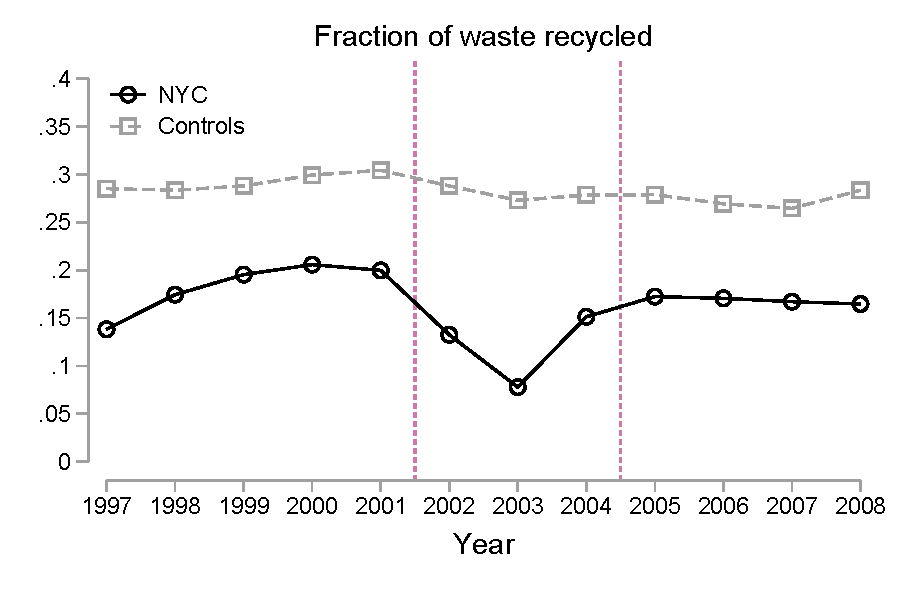
\includegraphics[width=0.7\textwidth]{rawparalleltrends.pdf}
    \caption{Recycling as a fraction of all waste in New York City and control regions in Massachusetts and New Jersey. Red vertical lines delineate the pause in metal, glass, and plastic recycling collection.}
    \label{fig:rawparalleltrends}
\end{figure}

The trends in figure \ref{fig:trends} appear consistent with a story of habit and skill formation in recycling that was interrupted by the cessation period, but when we compare these trends to control data, the story of habit and skill formation becomes less clear.  In figure \ref{fig:rawparalleltrends}, we plot the recycling rate in New York City boroughs and control regions.  In Massachusetts and New Jersey, the average recycling rate peaks in 2001 at 30\% and does not recover to this level during the 2002-2008 period, where the trend is relatively flat.  If the trends seen in Massachusetts and New Jersey generalize to New York City, the lower level of recycling in New York City after the cessation period may reflect overall trends in recycling rather than the effect of the cessation period.  We test this intuition formally with DID, synthetic control, and synthetic DID approaches in the following section.

\begin{table}
    \centering
    \begin{threeparttable}
    \caption{Comparison of New York City with controls}
    \label{tab:differenceinmeans}
    {\def\sym#1{\ifmmode^{#1}\else\(^{#1}\)\fi} \begin{tabular}{l*{3}{cc}} \hline
                    &\multicolumn{1}{c}{(1)}&\multicolumn{1}{c}{(2)}&\multicolumn{1}{c}{(3)}\\
                    &\multicolumn{1}{c}{NYC}&\multicolumn{1}{c}{Controls}&\multicolumn{1}{c}{Difference}\\
                    &     Mean/SD&     Mean/SD&Diff./t-stat         \\
\hline
Population, thousands&    1,995.73&      611.10&   -1,384.62\sym{***}\\
                    &    (482.43)&    (452.28)&    (-17.11)         \\
Income per capita   &   26,767.97&   39,215.74&   12,447.77\sym{***}\\
                    &  (4,836.11)&  (9,787.03)&     (15.00)         \\
Fraction nonwhite   &        0.72&        0.15&       -0.57\sym{***}\\
                    &      (0.10)&      (0.10)&    (-34.02)         \\
Fraction with college degree, 2000&        0.20&        0.32&        0.12\sym{***}\\
                    &      (0.04)&      (0.08)&     (16.75)         \\
Democratic presidential vote share, 2000&        0.81&        0.58&       -0.23\sym{***}\\
                    &      (0.05)&      (0.05)&    (-29.10)         \\
 & & & \\
N                   &          36&       2,484&       2,520         \\
Regions             &           3&         207&         210         \\
\hline\hline
\end{tabular}
}

    \begin{tablenotes}[flushleft]
    \scriptsize{Means and standard deviations are at the region level.  * \(p<0.05\), ** \(p<0.01\), *** \(p<0.001\)}
    \end{tablenotes}
    \end{threeparttable}
\end{table}

Finally, table \ref{tab:differenceinmeans} displays summary statistics comparing the New York City boroughs to the control regions in terms of income per capita, fraction nonwhite, fraction of residents with a college degree in 2000, and Democratic Party presidential vote share in 2000.\footnote{Population and income data are from the \cite{datacainc}, education data are from the United States Census and compiled by the \cite{dataeducation}, race data are from the \cite{datarace}, and vote share data are from \cite{datavoteshare}.}  On average, New York City differs from the controls in each of these measures, which may be related to the recycling rate.  This is a common concern in comparative case studies that we address in our analysis in several ways.  First, we test the robustness of our findings to controlling for these factors and find that they do not impact our estimates.  We further address this in our empirical strategy by using comparative case study methodologies such as synthetic control and synthetic DID approaches.  Ultimately, we are not concerned demographic differences are affecting the results, especially as we find that after the pause New York City recycling rate trends match the trends in the control regions---we would expect differences to cause a deviation in the recycling rates.

\section{Empirical strategy}

Our theoretical framework and plots of recycling over time suggest that recycling rates may have continued to increase during the pause in glass and plastic recycling collection.  In this section, we use DID, synthetic control, and synthetic DID approaches to estimate how recycling rates would have evolved if the recycling program had remained in continuous operation. We compare these synthetic counterfactuals to the actual evolution of New York City's recycling rate to estimate the effect of the cessation period.

We denote the recycling rate in region \(i = \lbrace 1,...,N \rbrace\) and year \(t = \lbrace 1997,...,2008 \rbrace\) as \(Y_{i,t}\).  The first \(N_{co}\) regions are control regions and the final \(N_{tr} = 3\) regions are treated regions so that \(N=N_{co}+N_{tr}\).  The binary treatment variable \(W_{i,t} \in \lbrace 0,1 \rbrace\) is equal to one for all New York City boroughs beginning in 2002 and is zero otherwise.\footnote{Thus, an \(N \times T\) matrix containing the values of \(W_{i,t}\) is lower block diagonal.}  We assume that the overall recycling rate follows the latent factor variable model:
\begin{align} \label{eq:factormodel}
    Y_{i,t} = \mu + \alpha_i + \beta_t + \sum_{t=2002}^{2008} W_{i,t} \tau_t + \varepsilon_{i,t},
\end{align}
where \(\mu\) is an intercept, \(\alpha_i\) are region-specific fixed effects, \(\beta_t\) are year-specific common shocks, and \(\varepsilon_{i,t}\) is conditional-mean-zero heterogeneity.  The effect of the pause in glass and plastic recycling collection potentially varies by year---the coefficients \(\tau = \tau_{2002},...,\tau_{2008}\) describe the dynamic treatment effect of the pause on recycling rates in New York City.  

Our goal is to recover estimates \(\hat{\tau} = \hat{\tau}_{2002},...,\hat{\tau}_{2008}\) of the effect of the pause on recycling rates in New York City.  Our hypotheses are that \(\tau_t < 0 \text{ } \forall \text{ } t\).  During the pause from 2002 to 2004, the treatment effect should mechanically be negative because glass and plastic were no longer accepted.  After the pause from 2005 to 2008, the treatment effect would be negative if the pause affected recycling habits and skills negatively.  We estimate \(\hat{\tau}\) using DID and synthetic DID approaches, which we describe in the following sections.  We present and discuss the results from each approach together in the next section.

\subsection{DID}

The leading approach to estimating \(\hat{\tau}\) is to estimate equation \ref{eq:factormodel} using ordinary least squares in a differences-in-differences event-study approach, often adding pre-treatment indicators to evaluate the presence of pre-trends.  Our first estimator follows \cite{borusyakjaravel2018} by estimating pre-trends and omitting the first and last pre-treatment period in the following model:
\begin{align} \label{eq:did}
    Y_{i,t} = \mu + \alpha_i + \beta_t + \sum_{\ell = 1998}^{2000} W_{i} \cdot 1(t=\ell) \tau_k^{pre} +  \sum_{\ell=2002}^{2008} W_{i} \cdot 1(t=\ell) \tau_\ell + X_{i,t}\gamma + \varepsilon_{i,t},
\end{align}
where \(W_i\) is a binary variable equal to one for regions in New York City and \(X_{i,t}\) are unit and time varying controls. The DID approach produces unbiased estimates of the treatment effects under standard parallel trends, no spillovers, and strict exogeneity assumptions. We control for per-capita income and fraction of non-white residents, but inclusion of these controls do not substantially change the estimates.\footnote{Estimating a model without pre-treatment leads (Borusyak and Jaravel's semi-dynamic specification) and only dropping one pre-treatment year produce similar estimates.}  

While we do not have reason to expect that there are spillovers or violations of the strict exogeneity assumption, it is not clear that there are parallel trends in the evolution of recycling rates in treatment and control groups.  Figure \ref{fig:rawparalleltrends} plots the outcome variable for Massachusetts and New York City during the study period.  Prior to 2002, the recycling rate in New York City rose at a faster rate relative to Massachusetts and New Jersey.  While the difference in trends is not egregious, we are cautiously concerned that the recycling rate in New York City may not have evolved similarly to the recycling rate in Massachusetts and New Jersey in the absence of the pause.  We now turn to methods such as synthetic control and synthetic DID that reweight the control units to match the pre-treatment evolution of the outcome variable.  Appendix section \ref{sec:sc} details a synthetic control approach that suffers from lack of precision due to poor pre-treatment fit.

\subsection{Synthetic DID}

Due to our concerns about the DID and synthetic control approaches, we turn to the synthetic DID approach introduced by \cite{arkhangelsky2021}.  The synthetic DID approach uses unit and time weights to create a synthetic control that exhibits parallel trends to the treated unit in the evolution of the outcome variable, allowing the researcher to conduct a DID-style analysis. In the canonical synthetic DID approach, the researcher is interested in estimating a single average treatment effect.  In our case, we are interested in estimating treatment effects by year, so we implement a ``stacked'' design that estimates a separate synthetic DID for each post-treatment year.  Let \(j \in \lbrace 2002,...,2008\rbrace\) index post-treatment years, and let \(\mathcal{T}_j =  \lbrace 1997,...,2001,j \rbrace\) be the set of pre-treatment years augmented with the post-treatment year \(j\).  We estimate the treatment effect \(\tau^{sdid}_j\) for each post-treatment year \(j\) using the synthetic DID-weighted regressions:
\begin{align} \label{eq:sdid}
     (\hat{\tau}^{sdid}_j,\hat{\mu},\hat{\alpha},\hat{\beta}) = \underset{\tau,\mu,\alpha,\beta}{\arg\min} \left\lbrace \sum_{i=1}^{N} \sum_{t \in \mathcal{T}_j}  \left( Y_{i,t} - \mu - \alpha_i - \beta_t - W_{i,t} \tau_j \right)^2 \hat{\omega}_i^{sdid} \hat{\lambda}_t^{sdid,j} \right\rbrace,
\end{align}
where \(\hat{\omega}_i^{sdid}\) and  \(\hat{\lambda}_t^{sdid,j}\) are the synthetic DID weights for post-treatment period \(j\).  For reference, we reproduce the definitions of the standard synthetic DID unit and time weights from \cite{arkhangelsky2021} in Appendix \ref{sec:weights}.

Note that the unit weights \(\hat{\omega}_i^{sdid}\) will not differ between each treatment effect estimate while the time weights \(\hat{\lambda}_t^{sdid,j}\) will differ.  This is because the unit weights try to create parallel trends between treatment and control in the pre-period (which does not depend on post-treatment data), while the time weights try to balance pre- and post-exposure periods which vary for each estimation depending on which post-treatment year we estimate weights for.  Intuitively, the synthetic DID unit weights are similar to synthetic control weights in that they create a more comparable treatment group, but unlike synthetic control weights they allow for a gap between treatment and control.  The time weights put more weight on pre-treatment periods that look similar to the post-treatment periods, which reduces variance.  By re-estimating weights for each treatment effect estimate of interest in the stacked approach, we put additional weight on the pre-treatment periods that are more relevant for each treatment effect rather than the average treatment, increasing the precision of the estimates.

\begin{figure}
\centering
\begin{subfigure}[t]{.49\textwidth}
    \centering
    \vspace{0pt}
     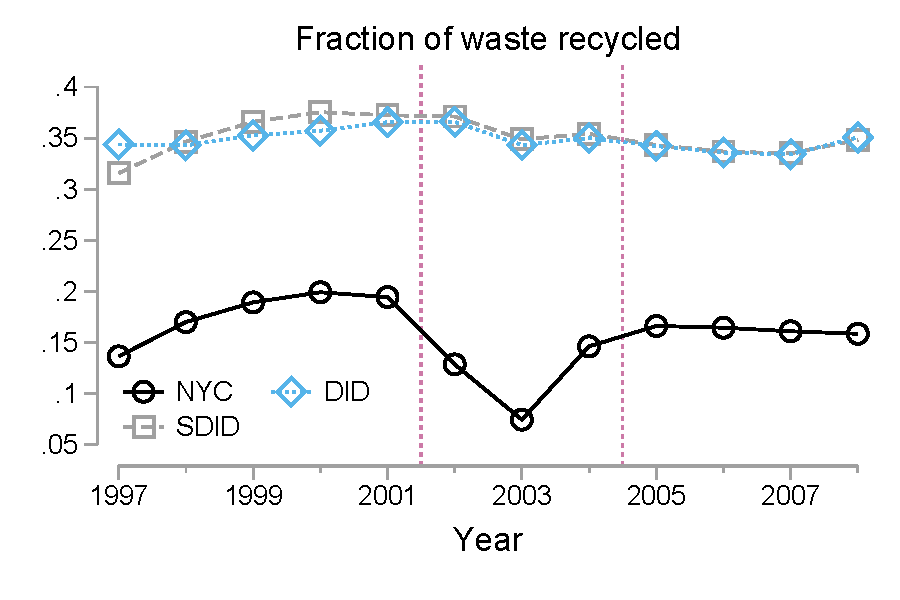
\includegraphics[width=\linewidth]{comparison.pdf}
        \caption{}\label{fig:comparisonpanel}
\end{subfigure}
    \begin{subfigure}[t]{.49\textwidth}
    \centering
    \vspace{0pt}
     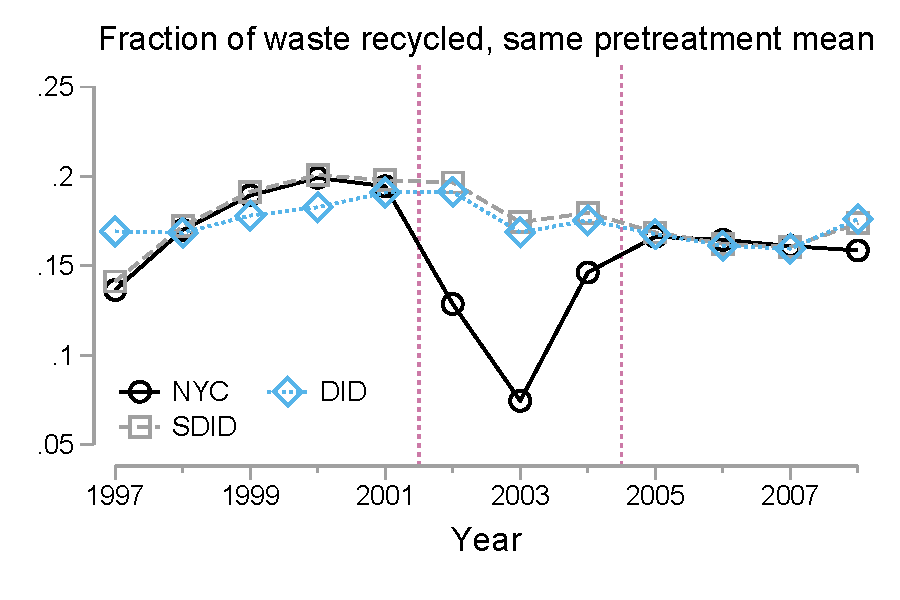
\includegraphics[width=\linewidth]{comparisonrecentered.pdf}
        \caption{}\label{fig:comparisonrecentered}
\end{subfigure}
    \caption{Panel (\subref{fig:comparisonpanel}) compares New York City's recycling rate with the DID control group, the synthetic control group, and the synthetic DID control group. Panel (\subref{fig:comparisonrecentered}) normalizes the pre-treatment mean of the DID and synthetic DID control groups to NYC's pre-treatment mean.} \label{fig:comparison}
\end{figure}

Figure \ref{fig:comparison} compares New York City's recycling rate with the DID control group, the synthetic control group, and the synthetic DID control group.\footnote{Because we create one synthetic DID control group for each post-treatment period, we plot the mean value of the synthetic DID control groups in the pre-treatment period.}  The synthetic DID reproduces the trends of the treated group and when recentered to the treated group's pre-treatment mean, it comes significantly closer than the synthetic control to matching the evolution of the outcome variable.  Interestingly, in the post-treatment time periods, the synthetic DID control group closely follows the DID control group, although the treatment effect estimates will still differ given the differences in the pre-treatment periods.

For a two-way fixed effects model like in equation \ref{eq:factormodel}, the synthetic DID approach returns consistent estimates of the treatment effect given uncorrelated and homoskedastic errors, sample size restrictions for convergence, and oracle weights that sum to one.\footnote{The sample size restrictions include asymptotically large pre-treatment periods and control units, larger number of control units relative to pretreatment periods, and larger number of control units than treated units.  See Theorem 1 and footnote 10 of \cite{arkhangelsky2021}.}  In small samples, the bias of the synthetic DID estimator is small when the weights are relatively evenly spread (or small), and when the weights are able to produce parallel trends in the outcome variable for treatment and synthetic control groups. Given the arbitrary nature of the pause in metal, glass, and plastic recycling, our small and evenly spread estimated weights (203 of 207 units are included in the final sample, with the largest weight not exceeding 0.015), and the ability of the weighted controls to produce parallel trends to the treatment group, we believe that our empirical context is well-suited to the synthetic DID approach.

An alternative approach is to include all post-treatment periods to estimate the weights and to estimate the treatment effect for each period in a joint estimation.  Between a joint and stacked approach, the unit weights differ only in that they are estimated with a larger regularization term in the joint synthetic DID relative to the stacked synthetic DID.\footnote{See equation \ref{eq:regularization}, where the regularization term \(\zeta\) depends on the length of the post period \(T_{post}\).}  Between the joint and stacked approach, the time weights differ because the joint synthetic DID is trying to weight pre-treatment periods that are similar to all post-treatment periods rather than balancing individually for each period in the stacked approach.  

\begin{figure}
\centering
\begin{subfigure}[t]{.49\textwidth}
    \centering
    \vspace{0pt}
     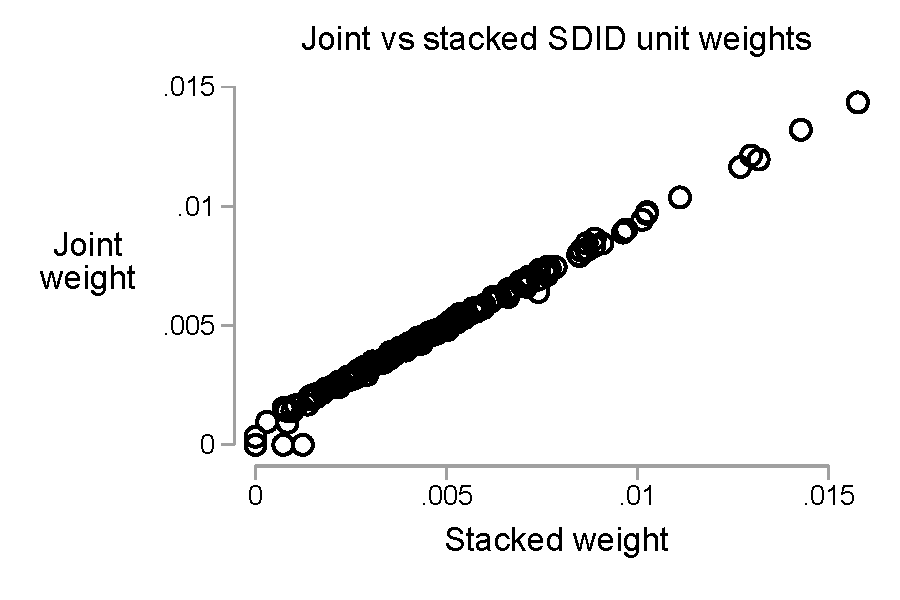
\includegraphics[width=\linewidth]{regionweights.pdf}
        \caption{}\label{fig:regionweights}
\end{subfigure}
    \begin{subfigure}[t]{.49\textwidth}
    \centering
    \vspace{0pt}
     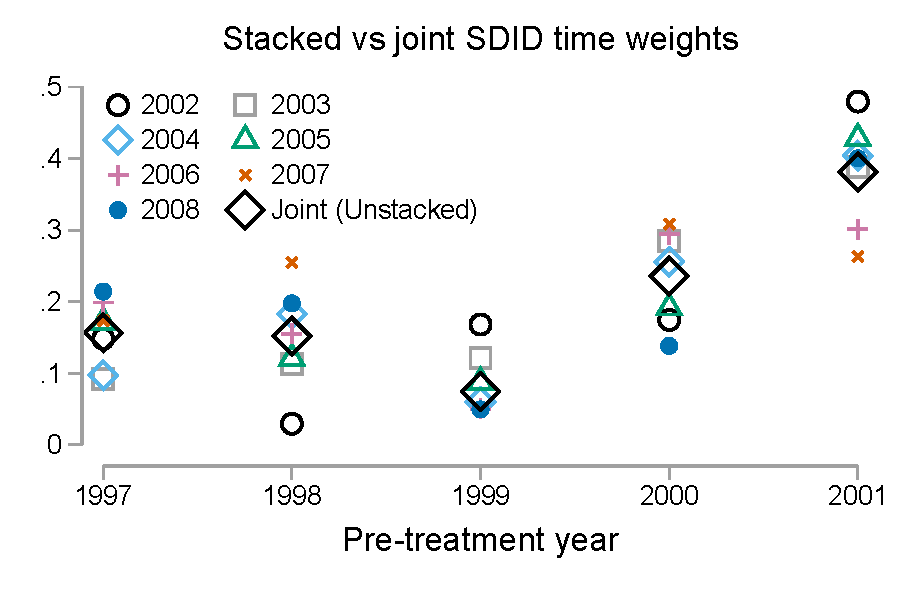
\includegraphics[width=\linewidth]{timeweights.pdf}
        \caption{}\label{fig:timeweights}
\end{subfigure}
    \caption{Panel (\subref{fig:regionweights}) compares unit weights and panel (\subref{fig:timeweights}) compares time weights from the stacked and joint synthetic DID procedures.} \label{fig:stackedjointcomparison}
\end{figure}

Mathematically, the joint time weights for each pre-treatment period are simply an average of the stacked weights.  We prove this formally in appendix section \ref{app:lseproof}, where the proof relies on the insight that the pre-period time weights are the solution to a penalized least-squares regression of the post-period outcomes on the pre-period outcomes and a constant, which allows us to apply a result from \cite{lawson1995}.  In figure \ref{fig:stackedjointcomparison}, we plot the time and region weights from the joint and stacked approaches in our empirical context.  Panel \ref{fig:regionweights} shows that the approaches produce similar region weights, but that the joint approach regularizes three region weights to zero due to the larger regularization term.  Panel \ref{fig:timeweights} shows that the time weights vary significantly for each stacked estimation.  For example, the weights on year 2000 vary from as much as 0.31 to 0.14 depending on which post-period coefficient we are estimating.  In Appendix \ref{sec:robustness}, we provide the estimates from the joint approach. We find that in our case, the two approaches produce similar point estimates but that the stacked approach provides more precise inference due to the time period rebalancing.  Because of this efficiency gain, we prefer the stacked synthetic DID approach and proceed to compare the stacked synthetic DID estimates to the event-study DID and synthetic control approaches in the next section.

\section{Results}

\begin{figure}
    \centering
    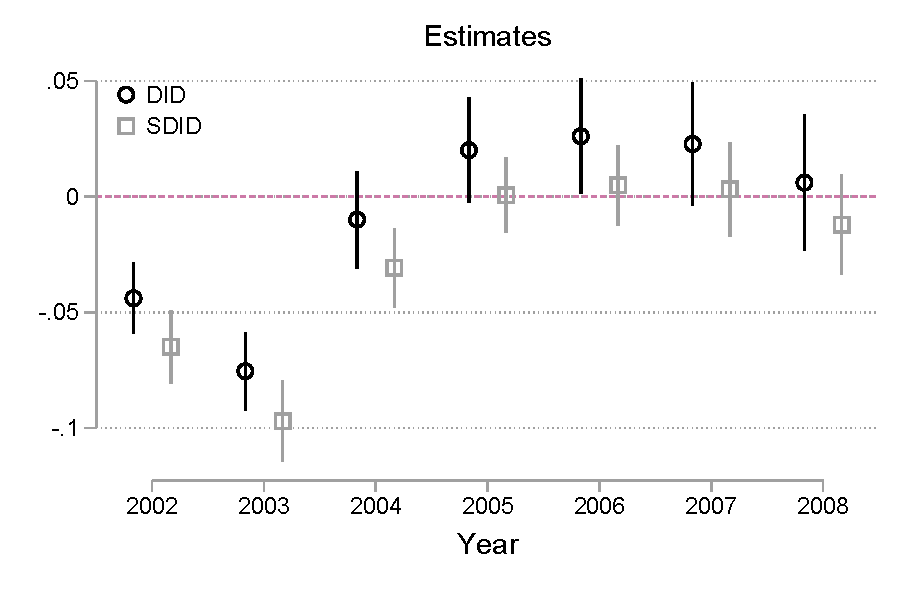
\includegraphics[width=0.8\textwidth]{estimates.pdf}
    \caption{Treatment effects of the 2002-2004 pause in metal, glass, and plastic collection by year using DID, synthetic control, and synthetic DID.  Confidence intervals are based on cluster-robust standard errors for DID and placebo-based inference for synthetic control and synthetic DID.}
    \label{fig:results}
\end{figure}

\begin{table}
    \centering
    \begin{threeparttable}
    \caption{Treatment effects by year and method}
    \label{tab:results}
    {
\def\sym#1{\ifmmode^{#1}\else\(^{#1}\)\fi}
\begin{tabular}{l*{2}{c}}
\hline\hline
          &\multicolumn{1}{c}{(1)}&\multicolumn{1}{c}{(2)}\\
          &\multicolumn{1}{c}{DID}&\multicolumn{1}{c}{SDID}\\
\hline
1998 X Treated&   0.0151\sym{**} &                  \\
          &  (0.005)         &                  \\
[1em]
1999 X Treated&   0.0278\sym{***}&                  \\
          &  (0.000)         &                  \\
[1em]
2000 X Treated&   0.0375\sym{***}&                  \\
          &  (0.000)         &                  \\
[1em]
2002 X Treated&  -0.0439\sym{***}&  -0.0649\sym{***}\\
          &  (0.000)         &  (0.000)         \\
[1em]
2003 X Treated&  -0.0754\sym{***}&  -0.0971\sym{***}\\
          &  (0.000)         &  (0.000)         \\
[1em]
2004 X Treated& -0.00989         &  -0.0306\sym{***}\\
          &  (0.353)         &  (0.000)         \\
[1em]
2005 X Treated&   0.0202         & 0.000599         \\
          &  (0.081)         &  (0.942)         \\
[1em]
2006 X Treated&   0.0262\sym{*}  &  0.00505         \\
          &  (0.039)         &  (0.567)         \\
[1em]
2007 X Treated&   0.0228         &  0.00322         \\
          &  (0.093)         &  (0.757)         \\
[1em]
2008 X Treated&  0.00612         &  -0.0120         \\
          &  (0.683)         &  (0.278)         \\
\hline
\(N\)     &     2520         &     2520         \\
Treated units&        3         &        3         \\
Control units&      207         &      207         \\
Controls selected&      207         &      203         \\
\hline\hline
\end{tabular}
}

    \begin{tablenotes}[flushleft]
    \scriptsize{P-values in parentheses based on cluster-robust standard errors at the region level for DID and placebo-based inference with placebo sampling at the region level for synthetic DID. * \(p<0.05\), ** \(p<0.01\), *** \(p<0.001\)}
    \end{tablenotes}
    \end{threeparttable}
\end{table}

Figure \ref{fig:results} and table \ref{tab:results} display the estimates from the DID and synthetic DID procedures.  For inference, we construct p-values using standard errors clustered at the region level for the DID estimates and use placebo-based inference p-values for the synthetic DID estimates.\footnote{We invert the p-values (using the assumption of a t-distribution) to create confidence intervals in the graphical display of the estimates for consistency, but one should be cautious in interpreting these given the nature of the treatment assignment in this comparative setting \citep{abadie2015}.}  The DID and synthetic DID approaches suggest that recycling levels dropped in response to the glass and plastic recycling pause, but recovered to their predicted levels in the first full year after resuming.

Our preferred synthetic DID estimates indicate that the pause in glass and plastic recycling collection reduced recycling rates by 6.5, 9.7, and 3.1 percentage points in 2002, 2003, and 2004 respectively.  In 2005, the first full year that recycling resumed, the synthetic DID estimate indicated that New York City's recycling rate was 0.06 percentage points \textit{higher} than the synthetic DID counterfactual prediction, suggesting a full recovery. From 2006 to 2008, our estimates indicate that recycling rates in New York City were unaffected by the pause, with all estimates close to zero in addition to including zero in the confidence interval.

In the appendix, we test the robustness of our findings to alternative modeling approaches. First, we test the robustness of synthetic DID to controlling for time- and unit-varying observable factors by partialing out control variables in a first stage.  The partialed synthetic DID estimates are slightly lower across the board, but are consistent with the main synthetic DID estimates.  Next, we implement a joint (or ``unstacked'') synthetic DID approach that uses one set of weights to estimate the dynamic treatment effects.  The joint synthetic DID point estimates are similar to the stacked synthetic DID point estimates but are substantially less precise.  Finally, given the fractional outcome variable, we propose and estimate an alternative correlated-random-effects fractional-response model following \cite{papkewooldridge2008}.  The fractional-response model estimates a larger reduction in recycling during the pause, but similarly shows a full recovery in recycling rates by 2005.  Overall, our results are robust to each of these alternative approaches.

In addition, we calculated the pre-treatment fit of each method using Cohen's \(d\), a unit-free measure of difference between the treatment group and its predicted counterfactual.  This statistic is often used to evaluate the quality of a matched control group in nearest-neighbor matching estimators and has been suggested as a way to evaluate the fit of synthetic controls, where lower values are preferred \citep{hollingsworth_wing_2020}. For each method, Cohen's \(d\) is defined as \(T_{pre}^{-1}\sum_{t\leq T_{pre}} N_{tr}^{-1}\sum_{i \geq N_{co}} (Y_{i,t}-\hat{Y}_{i,t})\sigma_i^{-1}\), the pre-treatment average difference between the recycling rate \(Y_{i,t}\) for the treated group minus the counterfactual predicted recycling rate \(\hat{Y}_{i,t}\), divided by the standard deviation of the pre-treatment recycling rate for unit \(i\), \(\sigma_i\).\footnote{For the synthetic DID approach, we compute the weighted average using the average estimated time weights used to construct the counterfactual \(\hat{\lambda}_t\).}  For example, the pre-treatment fit for the synthetic control approach is the value of synthetic New York's recycling rate, while the pre-treatment fit for the regression approach is the fitted values for the treated group from regression \ref{eq:did}.  As expected, the synthetic DID had the best pre-treatment fit (\(d\) = 0.24, and \(d\) = 0.22 with controls), followed by synthetic control (\(d\) = 0.46), the event-study (\(d\) = 0.51), and the fractional regression (\(d\) = 0.91).

Given the quick rebound in recycling rates, it does not appear that recycling habits and skills declined.  These results could be consistent either with persistent habits and skills or with a lack of habits and skills altogether.  Given the growth in recycling rates in New York City relative to Massachusetts from 1997-2002, it does appear that there is a learning-by-doing and habit-formation process taking place, so the recovery is more consistent with a persistent habits and skills explanation.  In the next section we examine mechanisms for the rebound in recycling rates and discuss how likely our findings are to generalize beyond New York City.

\section{Why did the recycling rate recover so quickly?}

The mechanisms allowing New York City's recycling rate to recover are important in determining when our results may generalize to other settings.  We examine several potential factors that may have contributed to the recovery of the recycling rate.  Given that the pause occurs only once in unique circumstances, it is difficult to formally test whether these mechanisms were pivotal in the recovery; however, we can marshal additional empirical and qualitative evidence to rule out some of these mechanisms.  We find little evidence that the rebound was driven by enforcement of the mandatory recycling law or the relative price of waste and recycling.  We find mixed evidence on the role of culture and environmental values.  Instead, we argue that habit and skill retention and persistence is the main mechanism driving the recovery, which was aided by the length of the pause relative to the age of the recycling program, continuity in other municipal waste collection programs, and the ease of recycling.  On the city's side, we note that the ability to terminate and quickly hire sanitation workers enabled a quick return to recycling.

First, we examine the role of the mandatory recycling law before and after the pause.  While recycling had been mandatory since 1989, enforcement of the requirement had not been substantially mentioned in DSNY reports and had not been listed as one of the top five sanitation violations until 2004 when glass and plastic recycling resumed.  In 2004, DSNY issued 35,674 notices of violation for failure to recycle.  This number increased to 47,443 in 2005.  In 2006, DSNY split recycling violations into categories of ``recyclables mixed with non-recyclables'' with 48,729 violations and ``non-recyclables in recyclable container'' with 46,644 violations---a doubling of enforcement two years after recycling resumed \citep{dsnyreports}.  However, a 2004-2005 study by DSNY estimated that only about 50\% of recyclable materials were actually recycled by New York City households \citep{dsnywcs2005}, which means that violations were commonplace among the 8 million residents.  In comparison, New York City officials issued 8.2 million parking tickets in 2002 and 9.6 million in 2004, so recycling enforcement is small when put into context with other commonplace municipal code enforcement \citep{nypost}.  In 2001 and 2005, the city conducted a survey of resident recycling behavior and found that in 2001 and 2005 that 53\% and 44\% of recycling households reported the mandatory recycling law as a reason for participation \citep{lange2007}.  The relatively low enforcement levels and decline in the reported importance of the mandatory recycling law is not consistent with the requirement playing an important role in the recovery.

In addition, New York City households are not simply substituting between recycling and non-recycling based on prices of the two options.\footnote{Thank you to an anonymous referee for making this point.} One common arrangement in cities with curbside residential waste pickup is that recycling is priced lower on a per-volume basis than landfill waste.  This price difference incentivizes diverting as much waste possible into the recycling bin (often, non-recyclable material is also illicitly placed into recycling bins).  In contrast, New York City, Boston, and Chicago are the only three major U.S. cities that fully fund solid waste management through city revenues rather than charging for waste \citep{cbcny2014}. Thus, a pricing mechanism was not likely driving the return to recycling.

We find mixed evidence on the role of recycling culture in preserving recycling rates despite the pause.  Prior to the pause, DSNY had invested in substantial public outreach regarding its recycling program \citep{dsnyreports}.  In 2002, a Pew survey found that 70\% of surveyed Americans reported recycling \citep{pew2009}.  Separate surveys conducted by the city in 2001 and 2005 found that 89\% and 85\% of surveyed New Yorkers reported recycling ``always'' or ``frequently'', with less than 4\% stating that they ``never'' recycle \citep{lange2007}.  Furthermore, in these surveys, New Yorkers estimated that they recycled 73\% and 81\% of all possible recyclable materials they discarded, when in reality, the city's estimated capture rate was closer to 50\% \citep{dsnywcs2005}.  While these numbers are likely inflated due to self-reporting bias, they are indicative of a strong culture around recycling both before and after the pause.  At the same time, the stated enthusiasm for recycling does not appear to translate into recycling behavior as the New York City recycling rate is much lower than the communities in Massachusetts and New Jersey.  For this reason, we see it as unlikely that recycling culture was a key factor in restoring recycling to its existing level.

We see persistent recycling habits and skills as the most likely explanation for the quick recovery in recycling rates.  In experimental psychology, one primary empirical test or measure of habits is whether automatic or habitual behavior continues in response to a cue even after the reward for the behavior has been removed \citep{dickinson1985,woodrunger2016}.  In the recycling context, this suggests that continued attempts to recycle by New York City residents after the beginning of the pause would be evidence of habits in recycling.  While we were unable to find systematic data to examine whether households continued to recycle after the pause, the sanitation commissioner John J. Doherty stated to the \textit{New York Times} that residents continued to place ``all kinds of junk'' in recycling bins at the beginning of the pause before getting used to the new recycling rules \citep{nytcardwell2002}.  In addition, DSNY's annual report from 2002-2003 stated that ``New Yorkers would have to change their habits of eight years, and there was neither time nor
advertising funds to retrain everyone overnight,'' when referring to the changes in recycling, which is evidence that DSNY managers believed that habits played a key role in recycling behavior.

Another important factor that makes the habit and skill retention story likely is the length of the pause. 
 The pause in glass and plastic recycling lasted for 21 months.  While this is a significant pause, the recycling program had existed since 1986 and had been mandatory for residents since 1989 \citep{lubasch1989,macbride2004}, so household habits and skills may have had substantial persistence over the relatively short cessation period.  In addition, recycling glass and plastic is relatively easy for households and thus not easily forgotten.  If recycling was complex, then observed outcomes might differ from what is seen in these data.  Furthermore, during the pause, paper, metal, and organic material collection continued, which may have helped to maintain habits and skills.  Given that the pause in glass and plastic recycling reduced paper and organic recycling by a small amount (figure \ref{fig:mgptrends}), the converse spillover may have helped to maintain habits and skills during the pause.  Continued complementary behaviors may reduce the cost of resuming a behavior after a pause.

As a final piece of evidence to support the habit and skill mechanism, we provide empirical estimates that recycling rates and levels in New York City are dynamically persistent from month to month.  In other words, we show that increases in recycling for a community district in one month predicts an increase in the following month.  While dynamic persistence is not itself a proof of habit or skill formation, it is consistent with this mechanism.  Formally, we seek to estimate the coefficient \(\rho\) in the following dynamic model:
\begin{align} \label{eq:arellanobond}
    Y_{d,m} = \rho Y_{d,m-1} + \alpha_d + \beta_m + u_{d,m},
\end{align}
where \(Y_{d,m}\) is a recycling rate or tonnage in New York City community district \(d\) and month \(m\), \(\alpha_d\) is district-specific heterogeneity, \(\beta_m\) is a common time shock, and \(u_{d,m}\) is the error term.  A positive estimate of \(\rho\) indicates dynamic persistence in recycling.  We estimate \(\rho\) from equation \ref{eq:arellanobond} by applying the first-differences GMM estimator of \cite{arellanobond1991} on all recycling, metal, glass, and plastic recycling, and paper and organics recycling for New York City districts before the pause.\footnote{The coefficients are the same sign and typically larger if applied to the entire sample period, but we focus on the pre-pause period to avoid any dynamic persistence that the pause may have induced.}  For each type of recycling, we use both the share and the tons of recycling collected as outcome variables and use the two-period lag as the exogenous predictor of the first lag in the Arellano-Bond framework.

Table \ref{tab:arellanobond} displays our estimates of the dynamic persistence coefficient \(\delta\) from equation \ref{eq:arellanobond}.  Each coefficient indicates dynamic persistence from month to month that is statistically different from zero, which can be interpreted that an increase in recycling in the previous month predicts an increase in recycling this month.\footnote{For each outcome, the Arellano-Bond autocorrelation test rejects the null hypothesis of zero autocorrelation in the first order first-differenced errors (\(p<0.001\)), indicating that including the lag in equation \ref{eq:arellanobond} is justified.  For each outcome except for tons of paper and organics, the Arellano-Bond autocorrelation test fails to reject the null hypothesis of zero autocorrelation in the second order first-differenced errors (\(p>0.1\)), suggesting the Arellano-Bond estimation approach is correctly specified.  For tons of paper and organics (table \ref{tab:arellanobond}, column 6), the second order test rejected the null hypothesis of zero autocorrelation (\(p=0.04\)), suggesting the Arellano-Bond approach may not be correctly specified.}  The converse is also true that a decrease in recycling in the previous month would predict a decrease in recycling this month.  This type of persistence is consistent with the mechanism of habit and skill formation.

\begin{table}
    \centering
    \begin{threeparttable}
    \caption{Arellano-Bond estimates of equation \ref{eq:arellanobond}}
    \label{tab:arellanobond}
    {
\def\sym#1{\ifmmode^{#1}\else\(^{#1}\)\fi}
\begin{tabular}{l*{6}{c}}
\hline\hline
          &\multicolumn{1}{c}{(1)}&\multicolumn{1}{c}{(2)}&\multicolumn{1}{c}{(3)}&\multicolumn{1}{c}{(4)}&\multicolumn{1}{c}{(5)}&\multicolumn{1}{c}{(6)}\\
          &\multicolumn{1}{c}{\shortstack{Recycling \\ share}}&\multicolumn{1}{c}{\shortstack{Recycling \\ tons}}&\multicolumn{1}{c}{\shortstack{Metal, glass, \\ plastic share}}&\multicolumn{1}{c}{\shortstack{Metal, glass, \\ plastic tons}}&\multicolumn{1}{c}{\shortstack{Paper, organics \\ share}}&\multicolumn{1}{c}{\shortstack{Paper, organics \\ tons}}\\
\hline
\(Y_{t-1}\)&    0.415\sym{***}&    0.201\sym{***}&    0.246\sym{***}&    0.368\sym{***}&    0.413\sym{***}&    0.231\sym{***}\\
          & (0.0296)         & (0.0240)         & (0.0668)         & (0.0637)         & (0.0310)         & (0.0286)         \\
\hline
\shortstack[l]{Time \\ indicators}&      Yes         &      Yes         &      Yes         &      Yes         &      Yes         &      Yes         \\
\shortstack[l]{First \\ differenced}&      Yes         &      Yes         &      Yes         &      Yes         &      Yes         &      Yes         \\
\shortstack[l]{Arellano \\ Bond}&      Yes         &      Yes         &      Yes         &      Yes         &      Yes         &      Yes         \\
N         &    2,552         &    2,552         &    2,552         &    2,552         &    2,552         &    2,552         \\
\hline\hline
\end{tabular}
}

    \begin{tablenotes}[flushleft]
    \scriptsize{Uses monthly data on recycling in New York City from before the pause. Standard errors cluster-robust to heteroskedasticity at the community district level. *** \(p<0.001\)}
    \end{tablenotes}
    \end{threeparttable}
\end{table}

On the city's side, DSNY was able to quickly scale up and down the size of the agency \citep{dsnyreports}.  From 2002-2004, the number of employees shrank by 9.4\%.  From 2004 to 2005, the number of employees grew by 2.7\%, including the hiring of 756 new sanitation workers and 78 new enforcement agents.  Given a strong labor market in the city, hiring new workers to expand capacity was not a barrier to resuming recycling after the pause.  DSNY also did not divest recycling collection capital during the pause, purchasing 17 collection trucks between 2002 and 2003 and 268 collection trucks in 2004 \citep{dsnyreports}.  A longer-lasting pause may have created barriers to resuming recycling that were not seen in the context of this natural experiment.

\section{Conclusions and policy implications}

This paper studies a pause in plastic and glass recycling collection in New York City from 2002-2004 using a DID event study, synthetic control, and synthetic DID approach.  We find that, relative to New Jersey and Massachusetts, recycling rates declined in New York City by 6.5, 9.7 and 3.1 percentage points from 2002-2004.  By 2005, however, the recycling rate had completely recovered as if the pause had not occurred.  These results suggest that recycling habits did not degrade during this temporary pause.  Thus, the opportunity cost of pausing recycling does not necessarily include lost habitual capital.  This is the first empirical test of the hypothesis that recycling habits will degrade if recycling programs are not maintained.

These findings are relevant during periods when commodity values are low or collection costs are high, which reduces the value of recycling.  For example, China's 2017 Operation National Sword policy restricted low-quality and food-contaminated recycling imports from other countries.  This restriction reduced China's imports of recyclable materials by 30\% \citep{linetal2023} and subsequently reduced the value of recyclable materials \citep{vedantametal2022}.  According to a Waste Dive database on municipal recycling programs, at least 118 municipal waste programs in the United States have ended or suspended recycling since 2018, most often citing costs and food contamination.  The database only reports six new programs opening during this period \citep{wastedive2023}.  While it is difficult to know how much of a change this is from previous periods, it suggests that for policymakers, the decision of whether to continue recycling is relevant.  Furthermore, some of the listed programs have continued to ask residents to separate materials for recycling even though those materials are collected and sent to a landfill.

The main policy implication of this paper is that a temporary pause in a municipal recycling program may not have long-term effects on household participation because of lost habits and skills.  During periods when the value of recycled materials is low, a temporary pause in a recycling program can alleviate budgetary pressure without incurring additional habitual or skill costs.  In addition, there may not be value in preserved skills and habits from asking residents to continue to separate different materials if those materials are ultimately sent to a landfill.

This does not imply that it is welfare-improving to pause recycling, which requires a much broader analysis of private and social costs and benefits. The full costs and benefits of a municipal recycling program include the net present value of current and future monetary costs and benefits, environmental (external) benefits, and existence value for the program.  Even if recycling is costly and habits and skills do not degrade, a pause may sacrifice environmental benefits and existence value.  A pause will also incur other direct costs.  For example, paying for public messaging materials to alert residents that the schedule has changed will be costly.  Furthermore, the value of recyclables may change shortly after the decision to pause recycling.  In the New York City case, the Mayor's office had expected \$40 million dollars per year in savings from the pause, but after the first year the program saved an estimated \$11 million \citep{nytsavings2003}.

One limitation of this study is the lack of available data on recycling contamination rates, so it is possible that the pause changed contamination rates even though the overall recycling rate returned to normal.  Finally, we note that in addition to the above factors that New York City is a unique and exceptional city.  While our findings of a quick and complete recovery in recycling rate are robust in this comparative case study, future analyses may show that habit persistence is context dependent.  As of 2021-2022, recycling rates in New York City are still around 20\% and overall US recycling rates have been fairly constant since the 2000s \citep{epa2022,catlinetal2021}, suggesting that household behavior and waste composition has not changed too substantially since the 2002-2004 pause.  Given that this is the first empirical evidence on the persistence of recycling habits and skills, the value of replication is high \citep{maniadistufanolist2017}. 

\bibliography{ref}
\bibliographystyle{chicago}

\clearpage

\appendix
\appendixpage

\section{Additional figures}

\begin{figure}[hb]
\centering
\begin{subfigure}[c]{.49\textwidth}
    \centering
    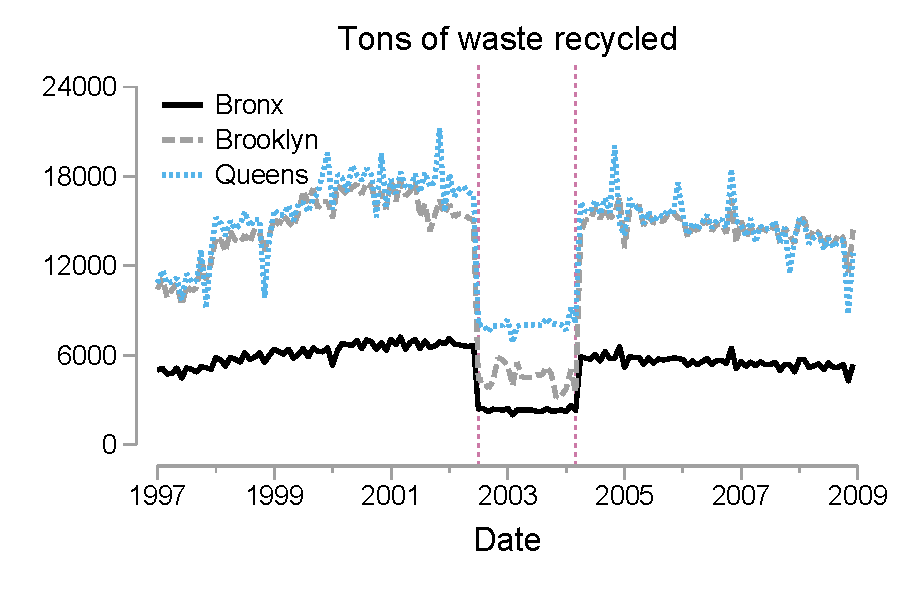
\includegraphics[width=\linewidth]{rr_level.pdf}
            \caption{}\label{fig:rr_level}
    \end{subfigure}
\begin{subfigure}[c]{.49\textwidth}
    \centering
    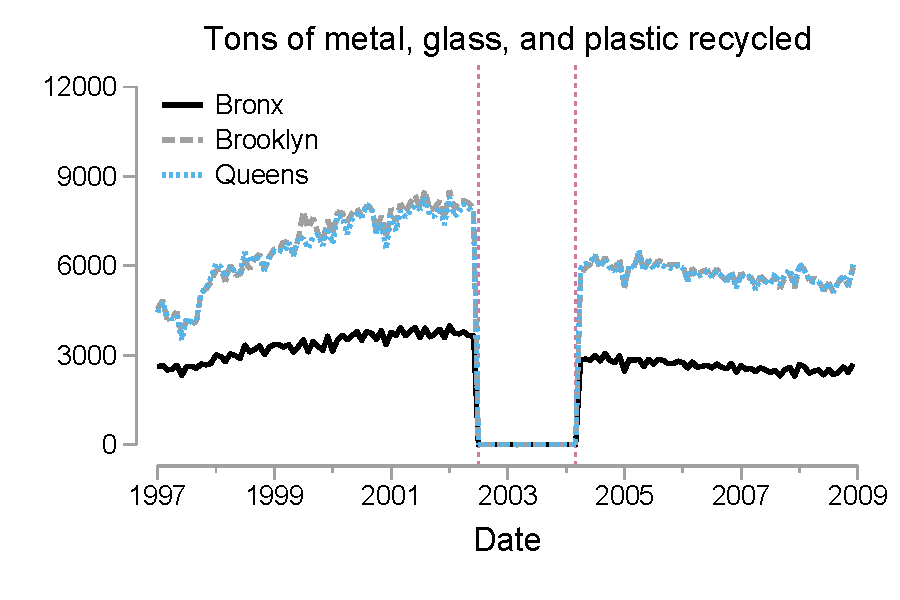
\includegraphics[width=\linewidth]{mgp_level.pdf}
        \caption{}\label{fig:mgp_level}
\end{subfigure}

\medskip

\begin{subfigure}[c]{.49\textwidth}
    \centering
    \vspace{0pt}
    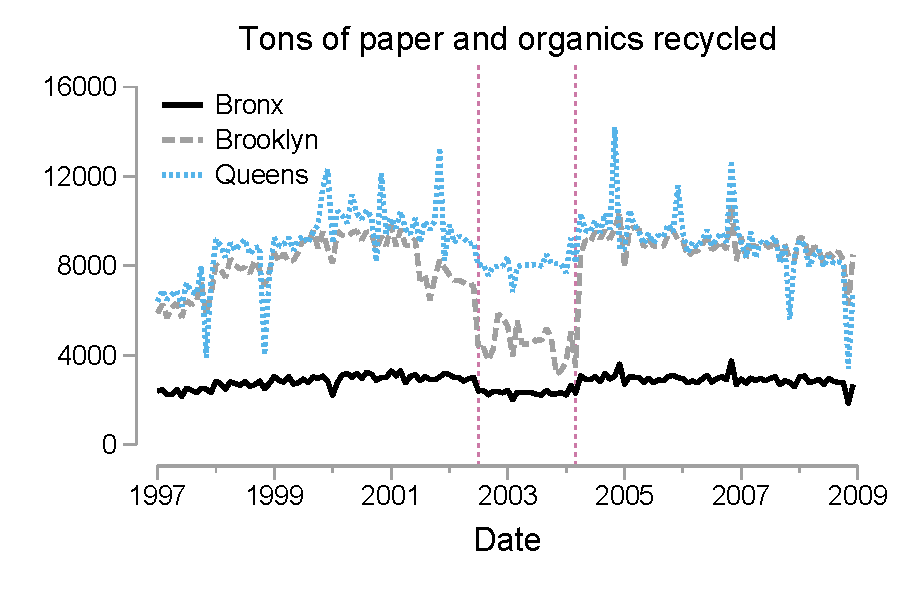
\includegraphics[width=\linewidth]{other_level.pdf}
        \caption{}\label{fig:other_level}
\end{subfigure}
\begin{subfigure}[c]{.49\textwidth}
    \centering
    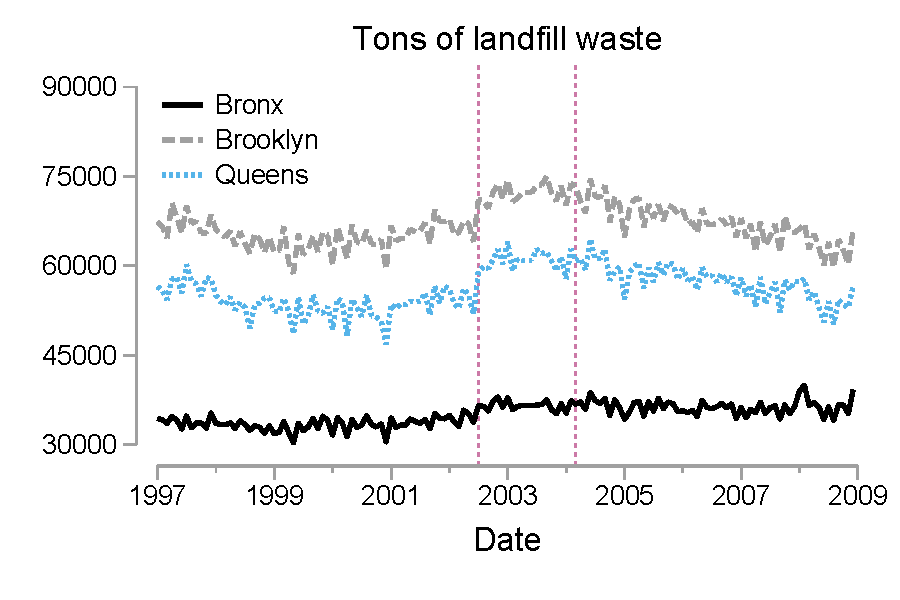
\includegraphics[width=\linewidth]{refuse_level.pdf}
        \caption{}\label{fig:refuse_level}
\end{subfigure}
    \caption{Deseasonalized monthly tons of waste disposed by type in New York City.  Red vertical lines delineate the pause in glass and plastic recycling collection.  Panel (\subref{fig:rr_level}) plots tons of all recycling, panel (\subref{fig:mgp_level}) plots tons of all metal, glass, and plastic recycling, panel (\subref{fig:other_level}) plots tons of paper and organics recycling, and panel (\subref{fig:refuse_level}) plots tons of all landfill waste. } \label{fig:trends_levels}
\end{figure}

\clearpage

\section{Synthetic DID weights} \label{sec:weights}

We reprise the synthetic DID weights from \cite{arkhangelsky2021} for reference.  Denote \(N\) the number of units and \(T\) the number of time periods, where the first \(N_{co}\) units are controls, and the last \(N_{tr}=N-N_{co}\) units are treated after time \(T_{pre}\).

The synthetic DID unit weights solve
\begin{align}
    (\hat{\omega}_0,\hat{\omega}^{sdid}) = \underset{\omega_0 \in \mathbb{R},\omega \in \Omega}{\arg\min} \quad f_{unit}(\omega_0,\omega)
\end{align}
where
\begin{align*}
    f_{unit}(\omega_0,\omega) = \sum_{t=1}^{T_{pre}}\left(\omega_0 + \sum_{i=1}^{N_{co}} \omega_i Y_{i,t} - \frac{1}{N_{tr}} \sum_{i=N_{co}+1}^N Y_{i,t}\right)^2 + \zeta^2 T_{pre} ||\omega ||^2_2, \\
    \Omega = \left\lbrace \omega \in \mathbb{R}_+^N: \sum_{i=1}^{N_{co}}\omega_i = 1, \quad \omega_i = N_{tr}^{-1} \text{ for all } i = N_{co}+1,...,N \right\rbrace
\end{align*}
where \(\mathbb{R}_+\) is the set of positive real numbers.  The regularization parameter is given by
\begin{align} \label{eq:regularization}
    \zeta = (N_{tr}T_{post})^{1/4}\hat{\sigma} \quad \text{ with } \quad \hat{\sigma}^2 = \frac{1}{N_{co}(T_{pre} - 1)} \sum_{i=1}^{N_{co}}\sum_{t=1}^{T_{pre} - 1} (\Delta_{i,t} - \bar{\Delta})^2,
\end{align}
with
\begin{align*}
    \Delta_{i,t} = Y_{i,(t+1)} - Y_{i,t} \quad \text{ and } \hat{\Delta} = \frac{1}{N_{co}(T_{pre}-1)} \sum_{i=1}^{N_{co}}\sum_{t=1}^{T_{pre} - 1} \Delta_{i,t}.
\end{align*}

The synthetic DID time weights solve
\begin{align}
     (\hat{\lambda}_0,\hat{\lambda}^{sdid}) = \underset{\lambda_0 \in \mathbb{R},\lambda \in \Lambda}{\arg\min} \quad f_{time}(\lambda_0,\lambda),
\end{align}
where
\begin{align*}
    f_{time}(\lambda_0,\lambda) =  \sum_{i=1}^{N_{co}}\left( \lambda _0 + \sum_{t=1}^{T_{pre}} \lambda_t Y_{i,t} - \frac{1}{T_{post}}\sum_{t=T_{pre}+1}^T Y_{i,t} \right)^2, \\
    \Lambda = \left\lbrace \lambda \in \mathbb{R}_+^{T}: \sum_{t=1}^{T_{pre}} \lambda_t = 1, \quad \lambda_t = T^{-1}_{post} \text{ for all } t = T_{pre}+1,...,T \right\rbrace.
\end{align*}

\section{Relationship between stacked and joint SDID weights} \label{app:lseproof}

In this section, we prove that the joint SDID pre-period time weights are a simple average of the stacked pre-period SDID weights.  Consider a general least squares regression problem with an equality constraint.  Denote a matrix of independent variables \(X\) as \(m_2 \times n\), a dependent variable \(Y\) as a vector of dimension \(n\), parameters \(\beta\) as a vector of dimension \(n\), \(C\) as a matrix of dimension \(m_1 \times n\), and \(d\) as a vector of dimension \(n\).  The least squares equality constraint problem is:
\begin{align}
    \underset{\beta}{\min} & \quad (X\beta - Y)'(X\beta - Y) \\ 
    & \text{s.t.} \quad C\beta = d
\end{align}
Note that the synthetic DID time weights fit in this class of minimization problems with \(Y = Y^{post}\), \(X =  Y^{pre}\), \(\beta = \lambda\) and constraint \(\sum_j \lambda_j = 1\).

\cite{lawson1995} suggests a method to derive the solution to this minimization problem by partitioning the data, constraint, and parameters to eliminate the constraint:
\begin{align}
    \left[ \begin{array}{c}
        C \\
        X
    \end{array} \right] = 
    \left[ \begin{array}{cc}
        C_1 & C_2 \\
        X_1 & X_2
    \end{array} \right],
\end{align}
where \(C_1\) is \(m_1 \times m_1\) and full rank, \(C_2\) is \(m_1 \times n-m_1\), \(X_1\) is \(m_1 \times m_2\), and \(X_2\) is \(n-m_1 \times m_2\). Furthermore,
\begin{align}
    \beta = 
    \left[ \begin{array}{c}
        \beta_1 \\
        \beta_2
    \end{array} \right],
\end{align}
where \(\beta_1\) is length \(m_1\) and \(\beta_2\) is length \(n-m_1\).  Solve the constraint for \(\beta_1\) to get \(\beta_1 = C_1^{-1}(d-C_2\beta_2)\) and substitute this into the objective function.  Rearrange terms to get an unconstrained least squares problem:
\begin{align}
    \underset{\beta_2}{\min} & \quad [(X_2 - X_1C_1^{-1}C_2)\beta_2-(Y-X_1C_1^{-1}d)]'[(X_2 - X_1C_1^{-1}C_2)\beta_2-(Y-X_1C_1^{-1}d)].
\end{align}
Simplify notation by denoting \(\Tilde{X} = (X_2 - X_1C_1^{-1}C_2)\) and \(\Tilde{a} = X_1C_1^{-1}d\) to rewrite the problem:
\begin{align}
    \underset{\beta_2}{\min} & \quad [\Tilde{X}\beta_2-(Y-\Tilde{a})]'[\Tilde{X}\beta_2-(Y-\Tilde{a})],
\end{align}
which has the familiar solution \(\beta_2^* = (\Tilde{X}'\Tilde{X})^{-1}\Tilde{X}'(Y-\Tilde{a})\).  Thus, any weight from the SDID procedure can be written in closed form as the solution to this unconstrained least squares problem.\footnote{Note that solving for \(\beta_1\) is simply substituting back into the constraint, but one may simply reorder the partition to see that any of the weights can be written this way.}  Each stacked SDID weight can be written as
\begin{align}
    \lambda^{stacked,j} = (\Tilde{X}'\Tilde{X})^{-1}\Tilde{X}'(Y_j-\Tilde{a}),
\end{align}
while the joint (unstacked) weights can be written as
\begin{align}
    \lambda^{joint} = (\Tilde{X}'\Tilde{X})^{-1}\Tilde{X}'(T^{-1}_{post} \sum_{j=1}^{T_{post}} [Y_j]-\Tilde{a}).
\end{align}
Note that \(\Tilde{a} = T^{-1}_{post} \sum_{j=1}^{T_{post}} \Tilde{a}\), which allows us to move \(\Tilde{a}\) into the summation.  We can pull \(T_{post}^{-1}\) out as a constant and can distribute terms to get 
\begin{align}
    \lambda^{joint} = T^{-1}_{post}\sum_{j=1}^{T_{post}}(\Tilde{X}'\Tilde{X})^{-1}\Tilde{X}'(Y_j-\Tilde{a}) = T^{-1}_{post}\sum_{j=1}^{T_{post}} \lambda^{stacked,j}.
\end{align}

\section{Robustness checks} \label{sec:robustness}

In this section, we test the robustness of our findings to alternative modeling approaches.  First, we partial out control variables in a step prior to estimating the treatment effects via the stacked DID approach.  Next, we consider a joint (unstacked) synthetic DID approach that uses one set of estimated synthetic DID weights to estimate all treatment effects.  Finally, we propose and estimate a correlated-random-effects fractional-response model following \cite{papkewooldridge2008} to account for the fractional outcome variable.  Each alternative approach yields estimates similar to our preferred synthetic DID estimates.

\begin{table}
    \centering
    \begin{threeparttable}
    \caption{Treatment effects by year and method}
    \label{tab:robustness}
    {
\def\sym#1{\ifmmode^{#1}\else\(^{#1}\)\fi}
\begin{tabular}{l*{4}{c}}
\hline\hline
          &\multicolumn{1}{c}{(1)}&\multicolumn{1}{c}{(2)}&\multicolumn{1}{c}{(3)}&\multicolumn{1}{c}{(4)}\\
          &\multicolumn{1}{c}{\shortstack{SDID\\Partialed}}&\multicolumn{1}{c}{\shortstack{SDID\\Unstacked}}&\multicolumn{1}{c}{\shortstack{Fractional\\DID}}&\multicolumn{1}{c}{\shortstack{Synthetic\\Control}}\\
\hline
1998 X Treated&                  &                  &   0.0172\sym{**} &                  \\
          &                  &                  &  (0.002)         &                  \\
[1em]
1999 X Treated&                  &                  &   0.0378\sym{***}&                  \\
          &                  &                  &  (0.000)         &                  \\
[1em]
2000 X Treated&                  &                  &   0.0508\sym{***}&                  \\
          &                  &                  &  (0.000)         &                  \\
[1em]
2002 X Treated&  -0.0664\sym{***}&  -0.0653         &  -0.0654\sym{***}& -0.00957         \\
          &  (0.000)         &  (0.066)         &  (0.000)         &  (0.870)         \\
[1em]
2003 X Treated&  -0.0991\sym{***}&  -0.0970\sym{**} &   -0.157\sym{***}&  -0.0611         \\
          &  (0.000)         &  (0.009)         &  (0.000)         &  (0.318)         \\
[1em]
2004 X Treated&  -0.0340\sym{***}&  -0.0309         &  -0.0200         &  -0.0541         \\
          &  (0.000)         &  (0.449)         &  (0.110)         &  (0.391)         \\
[1em]
2005 X Treated& -0.00526         &-0.000257         &   0.0206         &  -0.0273         \\
          &  (0.511)         &  (0.995)         &  (0.097)         &  (0.677)         \\
[1em]
2006 X Treated& -0.00313         &  0.00450         &   0.0256         &  -0.0609         \\
          &  (0.712)         &  (0.913)         &  (0.054)         &  (0.344)         \\
[1em]
2007 X Treated& -0.00579         &  0.00301         &   0.0204         &  -0.0115         \\
          &  (0.556)         &  (0.947)         &  (0.151)         &  (0.833)         \\
[1em]
2008 X Treated&  -0.0242\sym{*}  &  -0.0132         &  0.00229         &  -0.0579         \\
          &  (0.021)         &  (0.760)         &  (0.884)         &  (0.406)         \\
\hline
\(N\)     &     2520         &     2520         &     2520         &     2496         \\
Treated units&        3         &        3         &        3         &        1         \\
Control units&      207         &      207         &      207         &      207         \\
Controls selected&      202         &      201         &      207         &        2         \\
\hline\hline
\end{tabular}
}

    \begin{tablenotes}[flushleft]
    \scriptsize{Reports marginal effects from the fractional response DID regression.  P-values in parentheses based on cluster-robust standard errors for DID and placebo-based inference for synthetic control and synthetic DID. * \(p<0.05\), ** \(p<0.01\), *** \(p<0.001\)}
    \end{tablenotes}
    \end{threeparttable}
\end{table}

\subsection{Synthetic DID with controls}

\cite{arkhangelsky2021} suggest that one may include controls in the synthetic DID approach by using the Frisch-Waugh-Lovell theorem to partial out the effect of the controls on the outcome variable in a first stage.  In a first stage, we regress the recycling rate on per-capita income and fraction of non-white residents in region \(i\) in year \(t\) (the same control variables included in \(X_{i,t}\) in the DID regression in equation \ref{eq:did}).  Denote \(\Tilde{Y}_{i,t}\) the partialed outcomes.  We replace \(Y_{i,t}\) with \(\Tilde{Y}_{i,t}\) in equation \ref{eq:sdid} and estimate synthetic DID weights for each outcome in the stacked approach.

Column 1 in table \ref{tab:robustness} displays the results from the partialed out synthetic DID approach.  The estimates are more precise and slightly lower across the board relative to the stacked synthetic DID results in the main text, but do not tell a different story about the pause and recovery.

\subsection{Joint synthetic DID}

Next, we compare our stacked approach to a joint synthetic DID.  In this case, we estimate a single set of synthetic DID weights (\(\hat{\omega}_i^{joint},\hat{\lambda}_t^{joint}\)) using all of the post-treatment years.  The unit weights differ only in that they are estimated with a larger regularization term in the joint synthetic DID relative to the stacked synthetic DID.\footnote{See equation \ref{eq:regularization} in the appendix, where the regularization term \(\zeta\) depends on the length of the post period \(T_{post}\).}  The time weights will differ more because the joint synthetic DID is trying to weight pre-treatment periods that are similar to all post-treatment periods rather than balancing individually for each period in the stacked approach.  

After estimating the weights, we estimate the treatment effects of the pause using the synthetic DID-weighted regression:
\begin{align} \label{eq:sdidj}
     (\hat{\tau}_j,\hat{\mu},\hat{\alpha},\hat{\beta})^{joint} = \underset{\tau,\mu,\alpha,\beta}{\arg\min} \left\lbrace \sum_{i=1}^{N} \sum_{t=1997}^{2008}  \left( Y_{i,t} - \mu - \alpha_i - \beta_t - \sum_{t=2002}^{2008} W_{i,t} \tau_t \right)^2 \hat{\omega}_i^{joint} \hat{\lambda}_t^{joint} \right\rbrace.
\end{align}

Column 2 of table \ref{tab:robustness} displays the joint synthetic DID estimates.  The point estimates are very close to the stacked synthetic DID estimates in the main text, but are much less precise.  This is because one of the primary roles that the time weights play is to reduce the variance of the estimates.  This suggests that the stacked approach is more efficient for estimating dynamic treatment effects.

\subsection{Synthetic control} \label{sec:sc}

Given the potential lack of parallel trends, we also considered a synthetic control approach following \cite{abadie2021}.  We define \(Y_t\) as New York City's tonnage-weighted yearly average recycling rate for year \(t\).  Our synthetic control estimates \(\hat{\tau}_t^{sc}\) are:
\begin{align} \label{eq:sc}
    \hat{\tau_t}^{sc} = Y_t - \sum_{j=1}^{N_{co}} \omega^{sc}_j Y_{j,t}, \quad \forall \text{ } t \in \lbrace 2002,...,2008 \rbrace,
\end{align}
where \(\omega^{sc}_j\) are nonnegative synthetic control weights that sum to one and \(N_{co}\) is the number of control regions.  We choose the weights \(\hat{\omega}^{sc}_j\) so that:
\begin{align}
    \hat{\omega}^{sc} = \underset{\omega^{sc}}{\arg\min} \left\lbrace \sum_{h=1}^{k} \nu_h (X_h-\omega^{sc}_1 X_{h,1}-...-\omega^{sc}_{N_{co}} X_{h,N_{co}}) \right\rbrace,
\end{align}
where \((X_h,X_{h,1},...,X_{h,N_{co}})\) for \(h=1,...,k\) are the values of \(k\) matching variables for New York City and for the control regions.  The positive constants \(\nu_1,...,\nu_k\) reflect the relative importance of predictor \(h\) and are chosen to minimize the mean-squared prediction error between recycling rates in New York City and the control (donor) regions in the pre-period \citep{abadie2010}.\footnote{We estimate the synthetic control weights in Stata using the \verb+synth+ and \verb+synth_runner+ packages \citep{galianiquistorff2017}.}  For matching variables, we include the recycling rate from 1997 to 2001, year 2000 average education level and Democratic Party presidential vote share, and mean pre-intervention fraction of non-white residents and per-capita income.\footnote{A synthetic control using only pre-treatment outcomes does not look substantially different in this case.}  Intuitively, the synthetic control approach attempts to weight the control units to match New York City's recycling rate in the pre-period.

\begin{figure}
\centering
\begin{subfigure}[t]{.49\textwidth}
    \centering
    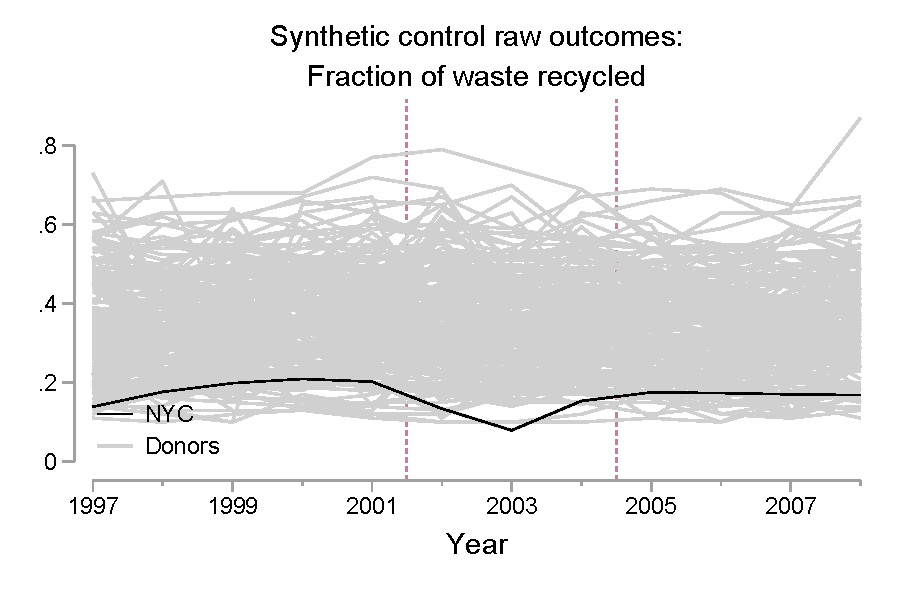
\includegraphics[width=\linewidth]{scrawoutcomes.pdf}
            \caption{}\label{fig:scrawoutcomes}
    \end{subfigure}
\begin{subfigure}[t]{.49\textwidth}
    \centering
    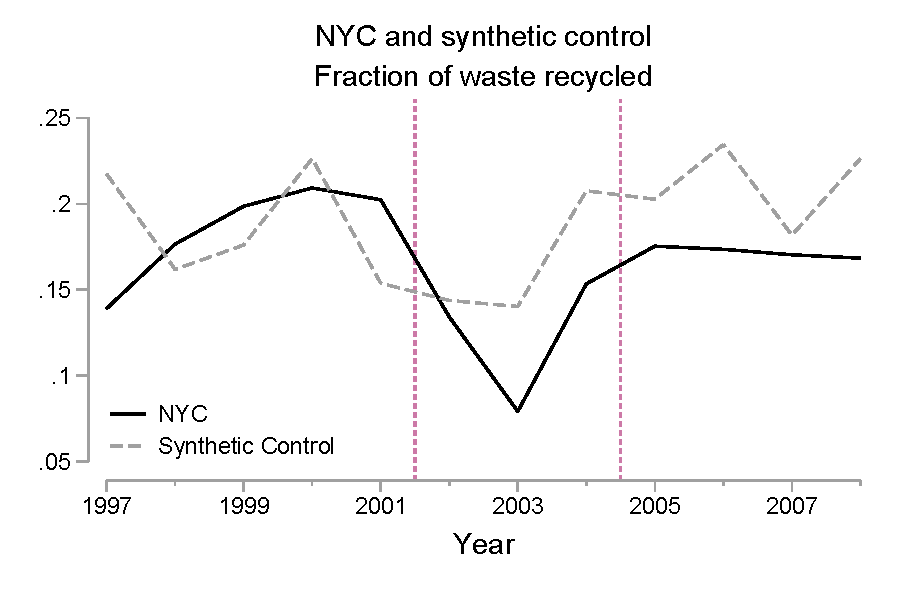
\includegraphics[width=\linewidth]{sctreatcontrol.pdf}
        \caption{}\label{fig:sctreatcontrol}
\end{subfigure} \\
\begin{subfigure}[t]{.49\textwidth}
    \centering
    \vspace{0pt}
     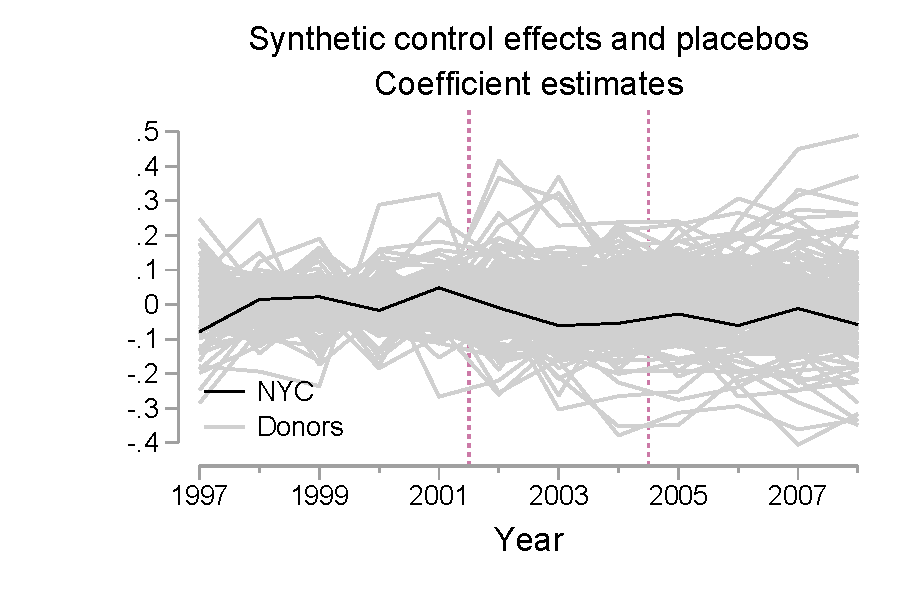
\includegraphics[width=\linewidth]{scplacebos.pdf}
        \caption{}\label{fig:scplacebos}
\end{subfigure}
\begin{minipage}[t]{.49\textwidth}
\medskip

\medskip
    \caption{Panel (\subref{fig:scrawoutcomes}) plots recycling rates for New York City and donor municipalities. Panel (\subref{fig:sctreatcontrol}) plots recycling rates for New York City and the synthetic control.  Panel (\subref{fig:scplacebos}) plots synthetic control estimates for New York City and placebo synthetic control estimates for the donor units.} \label{fig:sccomparison}
\end{minipage}
\end{figure}

The estimates in equation \ref{eq:sc} are unbiased in the case that our synthetic controls exactly reproduce the pre-intervention outcomes \citep{abadie2010}. When the pre-intervention outcomes do not match, the degree of bias is proportional to the ratio between the size of the heterogeneity \(\varepsilon_{i,t}\) and the length of the pre-treatment period.  In general, the difference between the synthetic control and treated unit outcomes in the pre-treatment period is an indication of the size of heterogeneity; thus, when the synthetic control is a good fit, the degree of bias is likely to be small \citep{abadie2021}.

Figure \ref{fig:scrawoutcomes} plots recycling rates for New York City and donor municipalities, and figure \ref{fig:sctreatcontrol} plots recycling rates for New York City and the synthetic control.  Our synthetic control weights are only nonzero for Boston, MA (0.414) and Hudson County, NJ (0.586).  The synthetic control recycling rate evolves somewhat similarly to New York City's, but does not match the pre-treatment values, particularly at the beginning and end of the pre-treatment period.  We believe that the synthetic control's inability to mimic New York City is a result of New York City's recycling rate being low relative to most of the control units, which can make it difficult for the synthetic control approximate \citep{abadie2021}.  The lack of good fit and the small number of pre-treatment periods point toward potential biases in the synthetic control outcomes. Figure \ref{fig:scplacebos} plots placebo synthetic control estimates for New York City and the donor units.  Even during the pause, the placebo estimates are often more extreme than the estimates for New York City, suggesting that the synthetic control estimates are imprecise and may largely reflect noise.  The results for the synthetic control model are in column 4 of table \ref{tab:robustness}, which are measured imprecisely.

\subsection{Fractional response model}

The DID event-study approach in equation \ref{eq:did} is valid for a continuous outcome variable; however, the recycling rate is limited to the \([0,1]\) interval.  Following \cite{papkewooldridge2008}, we can use the probit function to model the fractional recycling rate conditional expectation function:
\begin{align} \label{eq:fracreg}
    E[Y_{i,t}|\alpha_i,\beta_t,W_{i,t},X_{i,t}] = \Phi\left(\alpha_i + \beta_t + \sum_{\ell = 1998}^{2000} W_{i} \cdot 1(t=\ell) \tau_k^{pre} +  \sum_{\ell=2002}^{2008} W_{i} \cdot 1(t=\ell) \tau_\ell + X_{i,t}\gamma\right).
\end{align}
We can obtain consistent estimates of the coefficients and treatment effects (the marginal effects) using the Chamberlain-Mundlak device, which assumes that \(\beta_i = \psi + \bar{Z}_{i,t}\xi\), where \(Z_{i,t}=[W_{i,t},X_{i,t}]\) are the independent variables, \(\bar{Z}_{i,t}\) are the time averages of the independent variables, and \(\beta_i|Z_{i,t} \sim \text{Normal}(0,\sigma^2_\beta)\) where \(\sigma^2_\beta = Var(\beta_i|Z_{i,t})\).\footnote{The Chamberlain-Mundlak approach is necessary given the fixed effect \(\beta_i\), which cannot be consistently estimated due to the incidental parameters problem \citep{wooldridge2010}.}  Under these assumptions, we can estimate the conditional expectation function using probit quasi-maximum-likelihood estimation including time averages of the independent variables.

Column 3 of table \ref{tab:robustness} contains the treatment effects (the marginal effects) estimated using the fractional response model in equation \ref{eq:fracreg}.  The results display similar trends to the DID and synthetic DID estimates in the main text.  The main difference is that the fractional response model estimates a larger reduction in recycling rates during the pause in 2002 and 2003.  By 2004, the estimate of the effect of the pause is not statistically distinguishable from zero and is positive and not statistically distinguishable from zero in 2005-2008.  Overall, our findings in the main text are robust to estimating a fractional response model.
\end{document}

